%---------------------------------------------------------
\documentclass[a4paper,12pt]{report}

% --------------------
% LINGUA E CODIFICA
% --------------------
\usepackage[utf8]{inputenc}
\usepackage[T1]{fontenc}
\usepackage[italian]{babel}

% --------------------
% MATEMATICA
% --------------------
\usepackage{amsmath, amsfonts, amssymb, mathtools, mathrsfs, amsthm}
\usepackage[arrowdel]{physics}

% --------------------
% GRAFICA E FIGURE
% --------------------
\usepackage{graphicx}
\usepackage{float}
\usepackage{rotating}
\usepackage{dblfloatfix} % Figure doppie in fondo pagina
\usepackage{subcaption}
\usepackage[labelfont=bf]{caption}
\usepackage{forest}
\usepackage{array}

\usepackage{tikz}
\usetikzlibrary{arrows.meta, positioning, calc, fit}
% --------------------
% TABELLE
% --------------------
\usepackage{array, tabularx, multirow, longtable}
\newcolumntype{C}[1]{>{\centering\arraybackslash}p{#1}}
\renewcommand{\listtablename}{Tables}

% --------------------
% ALGORITMI E CODICE
% --------------------
\usepackage{listings}
\renewcommand{\listingscaption}{Codice}
% --------------------
% HYPERLINK
% --------------------
\usepackage{xcolor}
\usepackage{hyperref}

\AtBeginDocument{%
  \renewcommand{\sectionautorefname}{Sezione}
  \renewcommand{\subsectionautorefname}{Sezione}
  \renewcommand{\subsubsectionautorefname}{Sezione}
}
\providecommand*{\definitionautorefname}{Definizione}
\renewcommand{\figureautorefname}{Figura}
\renewcommand{\listingautorefname}{Codice}

\hypersetup{
    colorlinks,
    linkcolor={black!50!black},
    citecolor={black!50!black},
    urlcolor={blue!80!black}
}

% --------------------
% GEOMETRIA DELLA PAGINA
% --------------------
\usepackage[letterpaper,top=2cm,bottom=2cm,left=3cm]{geometry}

% --------------------
% PACCHETTI EXTRA
% --------------------
\usepackage{csquotes}
\usepackage{lipsum}
\usepackage[square]{natbib}
\usepackage{adjustbox}
\usepackage{textcomp, gensymb}
\usepackage[official]{eurosym}
\usepackage{cancel}
\usepackage{stmaryrd}
\usepackage{enumitem}

\usepackage{minted} 

% --------------------
% HEADER E FOOTER
% --------------------
\usepackage{fancyhdr}
\pagestyle{fancy}
\lhead{}
\chead{}
\rhead{}
\lfoot{}
\cfoot{\thepage}
\rfoot{}

\usepackage{tocloft}

% ---- Stile indice compatto ----
\setlength{\cftbeforesecskip}{5pt}    % niente spazio extra tra sezioni
\setlength{\cftbeforesubsecskip}{1pt} % niente spazio extra tra sottosezioni
\setlength{\cftbeforesubsubsecskip}{0pt}

% --------------------
% DEFINIZIONI PERSONALIZZATE
% --------------------
\newcommand\Set[2]{\{\,#1\mid#2\,\}}
\newcommand\SET[2]{\Set{#1}{\text{#2}}}

\graphicspath{{/images/}}

\makeatletter
\def\BState{\State\hskip-\ALG@thistlm}
\makeatother

\DeclareMathSizes{12}{12}{10}{8}
\usepackage{environ}
\usepackage[position=top]{subcaption}
\usepackage[most]{tcolorbox}

\usepackage{float}
\floatplacement{listing}{H}

\newcommand{\upperRomannumeral}[1]{\uppercase\expandafter{\romannumeral#1}}
\newcommand{\lowerromannumeral}[1]{\romannumeral#1\relax}

 % --- dimostrazione
\newenvironment{silentproof}{%
  \par\pushQED{\qed}\normalfont
}{%
  \popQED
}

% --------------------
% AUTORE E METADATI
% --------------------
\author{Ionut Georgian Zbirciog}

\hfuzz2pt % Ignora overfull < 2pt

\fancypagestyle{plain}{
  \fancyhead{}
  \renewcommand{\headrulewidth}{0pt}
}
\pagestyle{fancy}

\renewcommand{\sectionmark}[1]{\markright{\textit{#1}}{}}
\renewcommand{\subsectionmark}[1]{}

% --- NOTE SOTTO LA FOOTRULE ---
\makeatletter
\renewcommand{\footnoterule}{} % elimina la riga standard delle footnote

\def\@makecol{%
  \ifvoid\footins
    \setbox\@outputbox\box\@cclv
  \else
    \setbox\@outputbox\vbox{%
      \box\@cclv
    }%
  \fi
} 

\voffset=-5pt
\headsep=40pt
\hoffset=0pt
\textheight=620pt
\textwidth=435pt
\footskip=52pt

% --------------------
% HEADER E FOOTER (versione migliorata)
% --------------------
\fancyhead{}
\fancyfoot{}

% Titolo del capitolo a destra in alto
\fancyhead[R]{\leftmark}

% Numero di pagina centrato in basso
\fancyfoot[C]{\raisebox{-20pt}{\thepage}}

% Eventuali note o footnote a sinistra
\fancyfoot[L]{\parbox[b]{0.3\textwidth}{\unvbox\footins}}

% Linee di separazione
\renewcommand{\headrulewidth}{0.4pt}
\renewcommand{\footrulewidth}{0.4pt}

% --- Mostra il titolo del capitolo (non solo sezione) ---
\renewcommand{\chaptermark}[1]{\markboth{\textit{#1}}{}}
\renewcommand{\sectionmark}[1]{}

% Mantieni lo stile plain senza intestazione
\fancypagestyle{plain}{
  \fancyhead{}
  \renewcommand{\headrulewidth}{0pt}
}

\pagenumbering{arabic}

% --------------------
% AMBIENTI TEOREMI
% --------------------

\newtheorem{theorem}{Teorema}[section]

% Ambiente custom con titolo opzionale in grassetto
\makeatletter
\def\th@plain{%
  \thm@notefont{\bfseries}% <-- mette in grassetto la nota (cioè l'opzione [..])
  \itshape % corpo del teorema in corsivo
}
\makeatother

% --------------------
% AMBIENTI DEFINIZIONI
% --------------------
\newtheorem{definition}{Definizione}[section]
\renewcommand{\thedefinition}{\thesection.\arabic{definition}}

\NewDocumentEnvironment{de}{o}
  {\IfNoValueTF{#1}{\begin{definition}}{\begin{definition}[\textbf{#1}]}\normalfont}
  {\end{definition}}

% proposizione
\newtheorem{proposition}[theorem]{Proposizione}

% note
\newenvironment{note}[1]
  {\par\noindent\textbf{Nota (#1):}\ }
  {\par}


% --------------------
% STILE PARAGRAFI
% --------------------
\setlength{\parindent}{0pt}   % disattiva il rientro dei paragrafi
\setlength{\parskip}{0.5em}   % aggiunge spazio verticale tra paragrafi

% --------------------
% METADATI TESI
% --------------------
% intestazione.tex
\newcommand{\intestazione}{
    \thispagestyle{empty}
    %\vspace*{0.1cm} % Spazio in alto
    \begin{center}
        {\large \mytitle}
    \end{center}
    \begin{figure}[H]
        \centering
        
\includegraphics[height=3cm]{images/TorVergataLogo.png} % Sostituisci con il percorso corretto del logo
    \end{figure}
    \vspace{1cm} % Spazio tra il logo e il titolo
    \begin{center}
        {\large CORSO DI LAUREA IN\\
        \large \mycourse}
    \end{center}
    \vspace{1cm} 
    \begin{center}
        {\large TESI DI LAUREA IN\\
        \large \mytesi}
    \end{center}
    \vspace{1cm} 
    \begin{center}
        {\large TITOLO\\
        \large \mytesititolo}
    \end{center}
    \vfill
    \vspace{40pt}
    {\large
    \begin{tabbing}
    \hspace{12cm}\=\kill
    \textbf{Relatore:} \> \textbf{Candidato:} \\ % Prima riga con i titoli
    Prof. \> \mycandidato\\ % "Chiar.mo Prof." sotto la colonna "Relatore"
    \myrelatore  \> Matricola: \mymatricola 
    
    \end{tabbing}
    }
    \vspace{1.8cm} 
    \begin{center}
        {\normalsize Anno Accademico 2024/2025}
    \end{center}
    \newpage
}


\newcommand{\mytitle}{UNIVERSITÀ DEGLI STUDI DI ROMA TOR VERGATA\\\vspace{1cm}MACROAREA DI SCIENZE MATEMATICHE, FISICHE E NATURALI}
\newcommand{\mycourse}{INFORMATICA}
\newcommand{\mytesi}{ALGORITMI E STRUTTURE DATI}
\newcommand{\mytesititolo}{Progettazione e Sviluppo di un Sistema di Autenticazione Passwordless
Basato su Protocolli a Conoscenza Zero e Firme di Schnorr}
\newcommand{\myrelatore}{\textit{Francesco Pasquale}}
\newcommand{\mycandidato}{\textit{Ionut Georgian Zbirciog}}
\newcommand{\mymatricola}{\textit{0308984}}

% PROVA SCHEMA DB

\lstset{
  basicstyle=\ttfamily\footnotesize,
  columns=fullflexible,
  escapeinside={!}{!} % permette \tikzmark
}

\def\tikzmark#1{\tikz[overlay,remember picture]\node[inner sep=0pt,
 anchor=base](#1){\strut};}


\title{Tesi di Laurea in Informatica}
\author{Ionut Georgian Zbirciog}
\date{October 2025}

% --------------------
% DOCUMENTO
% --------------------
\begin{document}

\intestazione

\renewcommand{\contentsname}{}
\tableofcontents
\newpage
\thispagestyle{empty}
\null
\newpage
\chapter*{INTRODUZIONE}
\addcontentsline{toc}{chapter}{INTRODUZIONE}

% - Incipit con sistemi password-based
% - Obiettivo della tesi
% - Argomento di studio
% - Progetto

I sistemi di autenticazione più utilizzati attualmente sono quelli password-based. L'accesso a un account – che si tratti di \textit{Instagram}, \textit{Gmail} o di un portale universitario – richiede l'inserimento di un identificativo (username, email o matricola) abbinato a una \textbf{password}, ovvero una stringa alfanumerica creata al momento della registrazione.

In termini di \textit{user experience}, l'autenticazione basata su password risulta la soluzione più agevole, poiché richiede all'utente di memorizzare esclusivamente la password scelta in fase di registrazione. Nonostante ciò, il sistema è esposto a vulnerabilità: dalla perdita o dimenticanza della password, che impone una procedura di reimpostazione, fino alla possibilità che un attaccante la indovini (attacchi brute-force/enumerazione) o la intercetti, ottenendo accesso non autorizzato all'account.

La presente tesi ha come obiettivo la progettazione di un sistema (client-server) di autenticazione privo di password, fondato sull'utilizzo di un protocollo \textbf{Zero Knowledge Proof}, concetto introdotto per la prima volta alla fine degli anni '80 da Shafi Goldwasser, Silvio Micali e Charles Rackoff nel documento \textit{The Knowledge Complexity of Interactive Proof-Systems} \cite{doi:10.1137/0218012}. In particolare, verrà trattato il \textbf{Protocollo di Identificazione di Schnorr} e la relativa \textbf{Firma Digitale}, ideato da Claus Peter Schnorr alla fine degli anni '80 nel documento \textit{Efficient signature generation by smart cards} \cite{Schnorr2005}. A differenza dei meccanismi password-based, l'approccio \textit{ZKP} elimina la necessità di comunicare la password a ogni accesso, riducendo sia la probabilità di dimenticanza da parte dell'utente sia l'esposizione a rischi di sicurezza.

All'interno del protocollo d'identificazione di Schnorr, ciascun client dispone di una coppia di chiavi: la chiave pubblica $(pk := u)$ e la chiave segreta $(sk := \alpha)$.
Per garantire la sicurezza del protocollo, sia contro attacchi diretti sia contro tentativi di intercettazione, vengono impiegate operazioni modulari all'interno del gruppo crittografico $\mathbb{Z}_p$, con $p$ scelto come numero primo. I gruppi utilizzati seguono le specifiche dello standard RFC 3526 \cite{rfc3526}, il che implica che le chiavi avranno una lunghezza variabile a seconda della classe scelta (fino a 2048 bit nel caso del gruppo \texttt{modp-2048}, e così via).

Un punto cruciale è l'assunzione che il problema del logaritmo discreto (DL) sia computazionalmente \textbf{difficile} da risolvere. Si tratta di un problema matematico che, pur essendo facile da eseguire in una direzione, risulta estremamente complicato da invertire. Dato un gruppo moltiplicativo ciclico $G$ di ordine primo $q$, un generatore $g \in G$ e un elemento $u \in G$, il problema del logaritmo discreto consiste nel determinare l'esponente $\alpha \in \{0, \dots, q-1\}$ tale che 
\[
u = g^\alpha, \text{ dove } \alpha = \log_gu,
\]
dove $\alpha$ è appunto chiamato \textbf{logaritmo discreto} di $u$.

Poiché questo problema è considerato intrattabile con gli attuali metodi noti anche qualora un malintenzionato riuscisse a intercettare la chiave pubblica ($pk := g^\alpha$), non sarebbe comunque in grado di risalire in tempi utili alla corrispondente chiave privata ($sk := \alpha$).

Nel contesto di un protocollo di autenticazione si distinguono due entità principali: il \textbf{Prover} e il \textbf{Verifier}.
Il \textit{Prover} rappresenta il client, ossia l'entità software che consente all'utente di autenticarsi, mentre il \textit{Verifier} rappresenta il server, il quale ha il compito di validare tale autenticazione. In uno scenario di autenticazione \textit{passwordless} non viene utilizzata alcuna password tradizionale. Al contrario, il \textit{Prover} deve dimostrare al \textit{Verifier} di possedere una determinata chiave segreta associata al proprio account, ma senza mai trasmetterla direttamente. 

Il sistema sviluppato in questa tesi è basato sul \textbf{Protocollo di Autenticazione e Firma di Schnorr}. L'obiettivo è fornire un meccanismo di accesso sicuro che permetta all'utente di autenticarsi utilizzando esclusivamente il proprio \textit{username}, dimostrando il possesso della chiave segreta senza trasmetterla. Il sistema è implementato secondo un'architettura client-server, con un server sviluppato in \textit{Python} e un database \textit{MongoDB}, e prevede la gestione delle chiavi tramite operazioni di hashing (\texttt{SHA-256}) e cifratura (\texttt{AES-GCM}). Il protocollo di comunicazione, denominato \textbf{SAP (Schnorr-based Authentication Protocol)}, si articola in tre fasi principali: \textit{handshake}, \textit{registrazione/autenticazione} e \textit{accoppiamento di dispositivi}.

% Paragrafo per descrivere in sistesi il sistema implementato

Nonostante l'elevato livello di sicurezza garantito da questo approccio, nei sistemi reali si tende a preferire l'autenticazione tradizionale tramite password, ritenuta più agevole dal punto di vista della \textit{user experience}, pur a fronte della necessità di memorizzare la password stessa. Una delle principali criticità dei sistemi \textit{passwordless} risiede nel fatto che la chiave segreta è \textit{device-dependent/client-dependent}: essa deve infatti risiedere sul dispositivo o sul client utilizzato per l'accesso. Di conseguenza, la cancellazione accidentale della chiave da parte dell'utente comporterebbe l'impossibilità di autenticarsi. Uno degli obiettivi del sistema presentato in questa tesi è quello di mitigare tale limite introducendo un meccanismo di associazione di più dispositivi, sfruttando la \textbf{Firma Digitale di Schnorr}.

In conclusione, è stata realizzata un'applicazione multi-platform (Android, Linux, Windows) con \textit{Flutter}, che, tramite un'interfaccia grafica, rende più semplice l'utilizzo del sistema di autenticazione, mentre il client Linux sviluppato in \textit{Python} è disponibile esclusivamente in versione \texttt{CLI} (riga di comando).

La struttura del lavoro svolto è organizzata come segue:

\begin{itemize}
    \item \textbf{Capitolo 1 - Elementi di Aritmetica Modulare e Fondamenti di Crittografia} \\
    In questo capitolo vengono presentate le nozioni fondamentali di aritmetica modulare (definizione di gruppo, sottogruppo, etc...), insieme ad alcuni concetti chiave della crittografia, come il problema del logaritmo discreto, che costituiscono la base teorica del lavoro.
    \item \textbf{Capitolo 2 - Schnorr: Identificazione e Firma Digitale} \\
    Viene presentato il concetto di protocollo \textit{Zero-Knowledge Proof} e, successivamente, viene analizzato nel dettaglio il protocollo di identificazione di Schnorr e il relativo schema di firma digitale.
    \item \textbf{Capitolo 3 - Progetto Sperimentale - SchnorrAuthApp} \\
    È dedicato allo sviluppo del sistema di autenticazione \textit{passwordless} progettato nell'ambito di questa tesi, basato sul protocollo di identificazione e firma di Schnorr, con descrizione dell'architettura, del protocollo di comunicazione e dell'applicazione Flutter sviluppata.
    \item \textbf{Capitolo 4 - Conclusioni e Sviluppi Futuri} \\
    Riassume i risultati ottenuti e presenta alcune considerazioni sulle possibili estensioni e sviluppi futuri del progetto.
    \item \textbf{Appendice} \\
    Contiene frammenti di codice e implementazioni ritenute significative per la comprensione del sistema sviluppato.
\end{itemize}
\pagebreak
\chapter{Elementi di Aritmentica Modulare e Fondamenti di Crittografia}

In questo capitolo vengono presentate le nozioni fondamentali di aritmetica modulare insieme ad alcuni concetti chiave della crittografia presenti nel libro \textit{Cryptografy Theory and Practice} \cite{stinson2019cryptography} , che costituiranno la base teorica per l'analisi del protocollo di identificazione di Schnorr e per la progettazione del sistema di autenticazione che su di esso si fonda.

\section{Aritmetica Modulare}

\begin{de}[Congruenza]
	Siano $a \text{ e } b \in \mathbb{Z} \text{ e sia } m \in \mathbb{Z}^+. \\ \text{Scriviamo } a \equiv b \pmod{m} \Leftrightarrow m \text{ divide } b - a$ e si legge "$a$ è \textbf{congruente} a $b$ modulo $m$".
\end{de}

\begin{de}[Riduzione Modulare]
	Supponiamo di dividere $a \text{ e } b \text{ per } m$, \\ ottenendo quoziente e resto intero. Abbiamo quindi: \\
	$$a = q_1m + r_1 \text{ e } b = q_2m + r_2, \text{ dove } 0 \leq r_i \leq m - 1 \text{ e } i \in \{1, 2\}.$$
	
	Allora, $a \equiv b \pmod{m}\Leftrightarrow r_1 = r_2$. Scriveremo $r_1 \text{ come } a \pmod{m}$, ovvero il resto della divisione tra $a \text{ e } m$ e si legge "$a$ è \textbf{ridotto modulo} $m$".
\end{de}

\begin{de}[Aritmetica Modulo $m$]
	Definiamo aritmetica modulo $m$ \\ come:
	$$\mathbb{Z}_m = \{ 0, \ldots, m - 1 \}$$
	insieme a due operazioni, $+$ (addizione) e $\cdot$ (moltiplicazione). Tali operazioni \\ funzionano esattamente come la vera addizione e moltiplicazione ad eccezione dei risultati che sono ridotti modulo $m$.
	Ad esempio, se $m = 5$, allora $3 + 4 \equiv 2 \pmod{5}$ e $3 \cdot 4 \equiv 2 \pmod{5}$.
\end{de}

\subsection{Gruppi}

\begin{de}[Gruppo]
	Un \textbf{gruppo} è un coppia $G = (X, \star)$ dove $X$ è un insieme e $\star$ è l'operazione binaria definita su $X$, che soddisfa le seguenti proprietà:
	\begin{itemize}
		\item L'operazione $\star$ è \textbf{associativa}: $\forall\ a, b, c \in X,\ (a \star b) \star c = a \star (b \star c)$;
		\item Esiste l'elemento $id \in X$ chiamato \textbf{identità}, tale che $a \star id = id \star a = a,\ \forall\ a \in X$;
		\item $\forall\ a \in X,\ \exists\ b\in X$ chiamato \textbf{inverso} di $a$, tale che $a \star b = b \star a = id$.
	\end{itemize}
\end{de}

\begin{de}
	Un gruppo $G = (X, \star)$ è \textbf{abeliano} se l'operazione $\star$ è \textbf{commutativa}, ovvero $a \star b = b \star a,\ \forall\ a,b \in X $.
\end{de}

\begin{de}
	Un gruppo $G = (X, \star)$ è \textbf{finito} se l'insieme $X$ è finito.
\end{de}

\begin{de}
	L'\textbf{ordine} di un gruppo finito $G = (X, \star)$, indicato con $ord(G)$, è uguale a $|X|$.
\end{de}

\begin{de}[Sottogruppo]
    Sia $G = (X, \star)$ un gruppo finito e sia $Y \subseteq X$. Allora diremo che $H = (Y, \star)$ è un \textbf{sottogruppo} di $G$ se $H$ è anch'esso un gruppo finito.
\end{de}

\begin{theorem}
    Sia $G = (X, \star)$ un gruppo finito e sia $Y \subseteq X$. Allora diremo che $H = (Y, \star)$ è un \textbf{sottogruppo} di $G$ se $H$ è \textbf{chiuso} rispetto l'operazione $\star$, ovvero se $\forall\ h_1,\ h_2 \in H,\ h1 \star h2 \in H$.
\end{theorem}

\begin{theorem}[Teorema di Lagrange]\label{thm:lagrange}
    Sia $H = (Y, \star)$ un sottogruppo finito del gruppo $G = (X, \star)$.
    Allora $\textbf{ord}(H) \text{ divide } \textbf{ord}(G)$.
\end{theorem}

\begin{de}[Gruppo additivo $\mathbb{Z}_n$] Sia $n \geq 2$ un intero. Allora la coppia $(\mathbb{Z}_n, +)$ è un gruppo abeliano finito di ordine $n$, dove il $+$ indica l'operazione di addizione modulo $n$. L'elemento identità è $0$ e l'inverso di un elemento $a \in \mathbb{Z}_n \text{ è } (-a) \pmod{n}$. 
\end{de}

\begin{de}[Gruppo moltiplicativo $\mathbb{Z}_p^\ast$] Sia $p \geq 2$ primo.\\ Definiamo $\mathbb{Z}_p^\ast = \mathbb{Z}_p \setminus \{0\}$. Allora $(\mathbb{Z}_p^\ast, \cdot)$ è un gruppo finito abeliano di ordine $p - 1$, dove $\cdot$ indica l'operazione di moltiplicazione modulo $p$. L'elemento identità è $1$ e l'inverso di un elemento $a \in \mathbb{Z}_p^\ast \text{ è } a^{-1}$.
\end{de}

\begin{de}[Ordini degli Elementi del Gruppo] Dato un gruppo finito $(X, \star)$, definiamo \textbf{ordine} di un elemento $a \in X$, indicato con $\mathbf{ord}(a)$, il più piccolo intero $m$ tale che
	$$\underbrace{a \star a \star \ldots \star a}_{m} = id$$
	In base alla tipologia di operazione che assume $\star$, si ha
	\[
		\underbrace{a \star a \star \ldots \star a}_{m} =
		\begin{cases}
			a^m & \text{se l'operazione è scritta in forma moltiplicativa}, \\[6pt]
			am  & \text{se l'operazione è scritta in forma additiva}.       
		\end{cases}
	\]
	L'elemento identità ha ordine $1$ mentre qualsiasi altro elemento diverso dall'identità ha ordine maggiore di $1$.
	Per esempio, nel gruppo $(\mathbb{Z}_n, +)$, l'elemento $1$ ha ordine $n$.
\end{de}

\subsection{Gruppi Ciclici ed Elementi Primitivi}

\begin{de}[Gruppo Ciclico]\label{def:gruppo_ciclico} Un gruppo abeliano finito $(X, \star)$ è un \textbf{gruppo ciclico} se esiste un elemento $a \in X$ avente ordine uguale a $|X|$. Tale elemento è chiamato \textbf{generatore} del gruppo.
	
	Ad esempio, sia $p \geq 2$ primo. Allora $(\mathbb{Z}_p^\ast, \cdot)$ è un gruppo ciclico di ordine $p - 1$, e un generatore di questo gruppo è chiamato \textbf{elemento primitivo modulo} $p$.\\
	In altre parole, esiste $g \in \mathbb{Z}_p^\ast$, tale che $\mathbb{Z}_p^\ast := \{1, g, g^2, g^3, \ldots, g^{p-2}\}$.\\
	Per esempio, in $\mathbb{Z}_7^\ast:\ \langle3\rangle := \{1, 3, 3^2, 3^3, 3^4, 3^5\} = \{1, 3, 2, 6, 4, 5\} \pmod{7} = \mathbb{Z}_7^\ast$.
\end{de}

\begin{de}
    Sia $G = (X, \star)$ un gruppo finito e sia $a \in X$. Definiamo
    \[
    \langle a \rangle := \{a^i: i \geq 0\}.
    \]
    È facile da dimostrare che $(\langle a \rangle, \star)$ è un sottogruppo di $G$, che è ciclico e che $\mathbf{ord}(\langle a \rangle) = \mathbf{ord}(a)$. Il sottogruppo $(\langle a \rangle, \star)$ è chiamato \textbf{sottogruppo generato da} $a$ e per il \autoref{thm:lagrange}, $\mathbf{ord}(\langle a \rangle) \mid \mathbf{ord}(G)$. 
\end{de}

\section{Logaritmo Discreto}\label{sec:dl}

In questa sezione si va a definire il problema del logaritmo discreto (DL Problem) e del perché è fondamentale per la maggior parte dei protocolli di crittografia.
Iniziamo con definire tale problema per un gruppo moltiplicativo finito generico $(G, \cdot)$. Scelto un elemento (generatore) $\alpha \in G$ avente ordine $n$, definiamo:
$$\langle\alpha\rangle := \{ \alpha^i: 0 \leq i \leq n - 1 \}$$
È facile da dimostrare che $\langle\alpha\rangle$ è un sottogruppo di $G$, che è ciclico ed ha ordine $n$.

Più nello specifico, il gruppo moltiplicativo maggiormente usato è $(\mathbb{Z}_p^\ast, \cdot)$ con $p$ primo e ordine $q$ anch'esso primo, tale che $p - 1 \equiv 0 \pmod{q}$. Si sceglie poi un generatore $\alpha \in \mathbb{Z}_p^\ast$ avente ordine primo $q$ nel seguente modo: preso un qualsiasi elemento primitivo in $\mathbb{Z}_p^\ast$ lo si eleva alla $\frac{(p - 1)}{q}$ potenza, determinando:
$$\langle\alpha\rangle := \{ \alpha^i: 0 \leq i \leq q - 1 \}$$

\begin{de}[Logaritmo Discreto]
	Sia $(G, \cdot)$ un gruppo moltiplicativo finito, sia $\alpha \in G$ avente ordine $n$ e sia $\beta \in \langle\alpha\rangle$. Il problema del \textbf{logaritmo discreto} consiste nel trovare l'unico intero $a,\ 0 \leq a \leq n - 1$ tale che 
	$$\alpha^a = \beta$$
	ovvero $a = \log_\alpha{\beta}$ ed è appunto chiamato \textbf{logaritmo discreto} di $\beta$.
\end{de}

L'ampio utilizzo del logaritmo discreto in crittografia deriva dal fatto che il problema di calcolarlo è considerato computazionalmente difficile, cioè non si conoscono algoritmi efficienti in grado di risolverlo in tempi ragionevoli. Al contrario, l'operazione inversa, ossia l'elevamento a potenza modulo un numero, può essere eseguita in maniera estremamente rapida grazie ad algoritmi ottimizzati come l'esponenziazione modulare. Questa asimmetria tra la facilità del calcolo diretto e la difficoltà apparente del problema inverso è ciò che conferisce sicurezza a molti protocolli crittografici basati sul logaritmo discreto.

\begin{figure}[H]
  \centering
  \begin{subfigure}{0.48\textwidth}
    \centering
    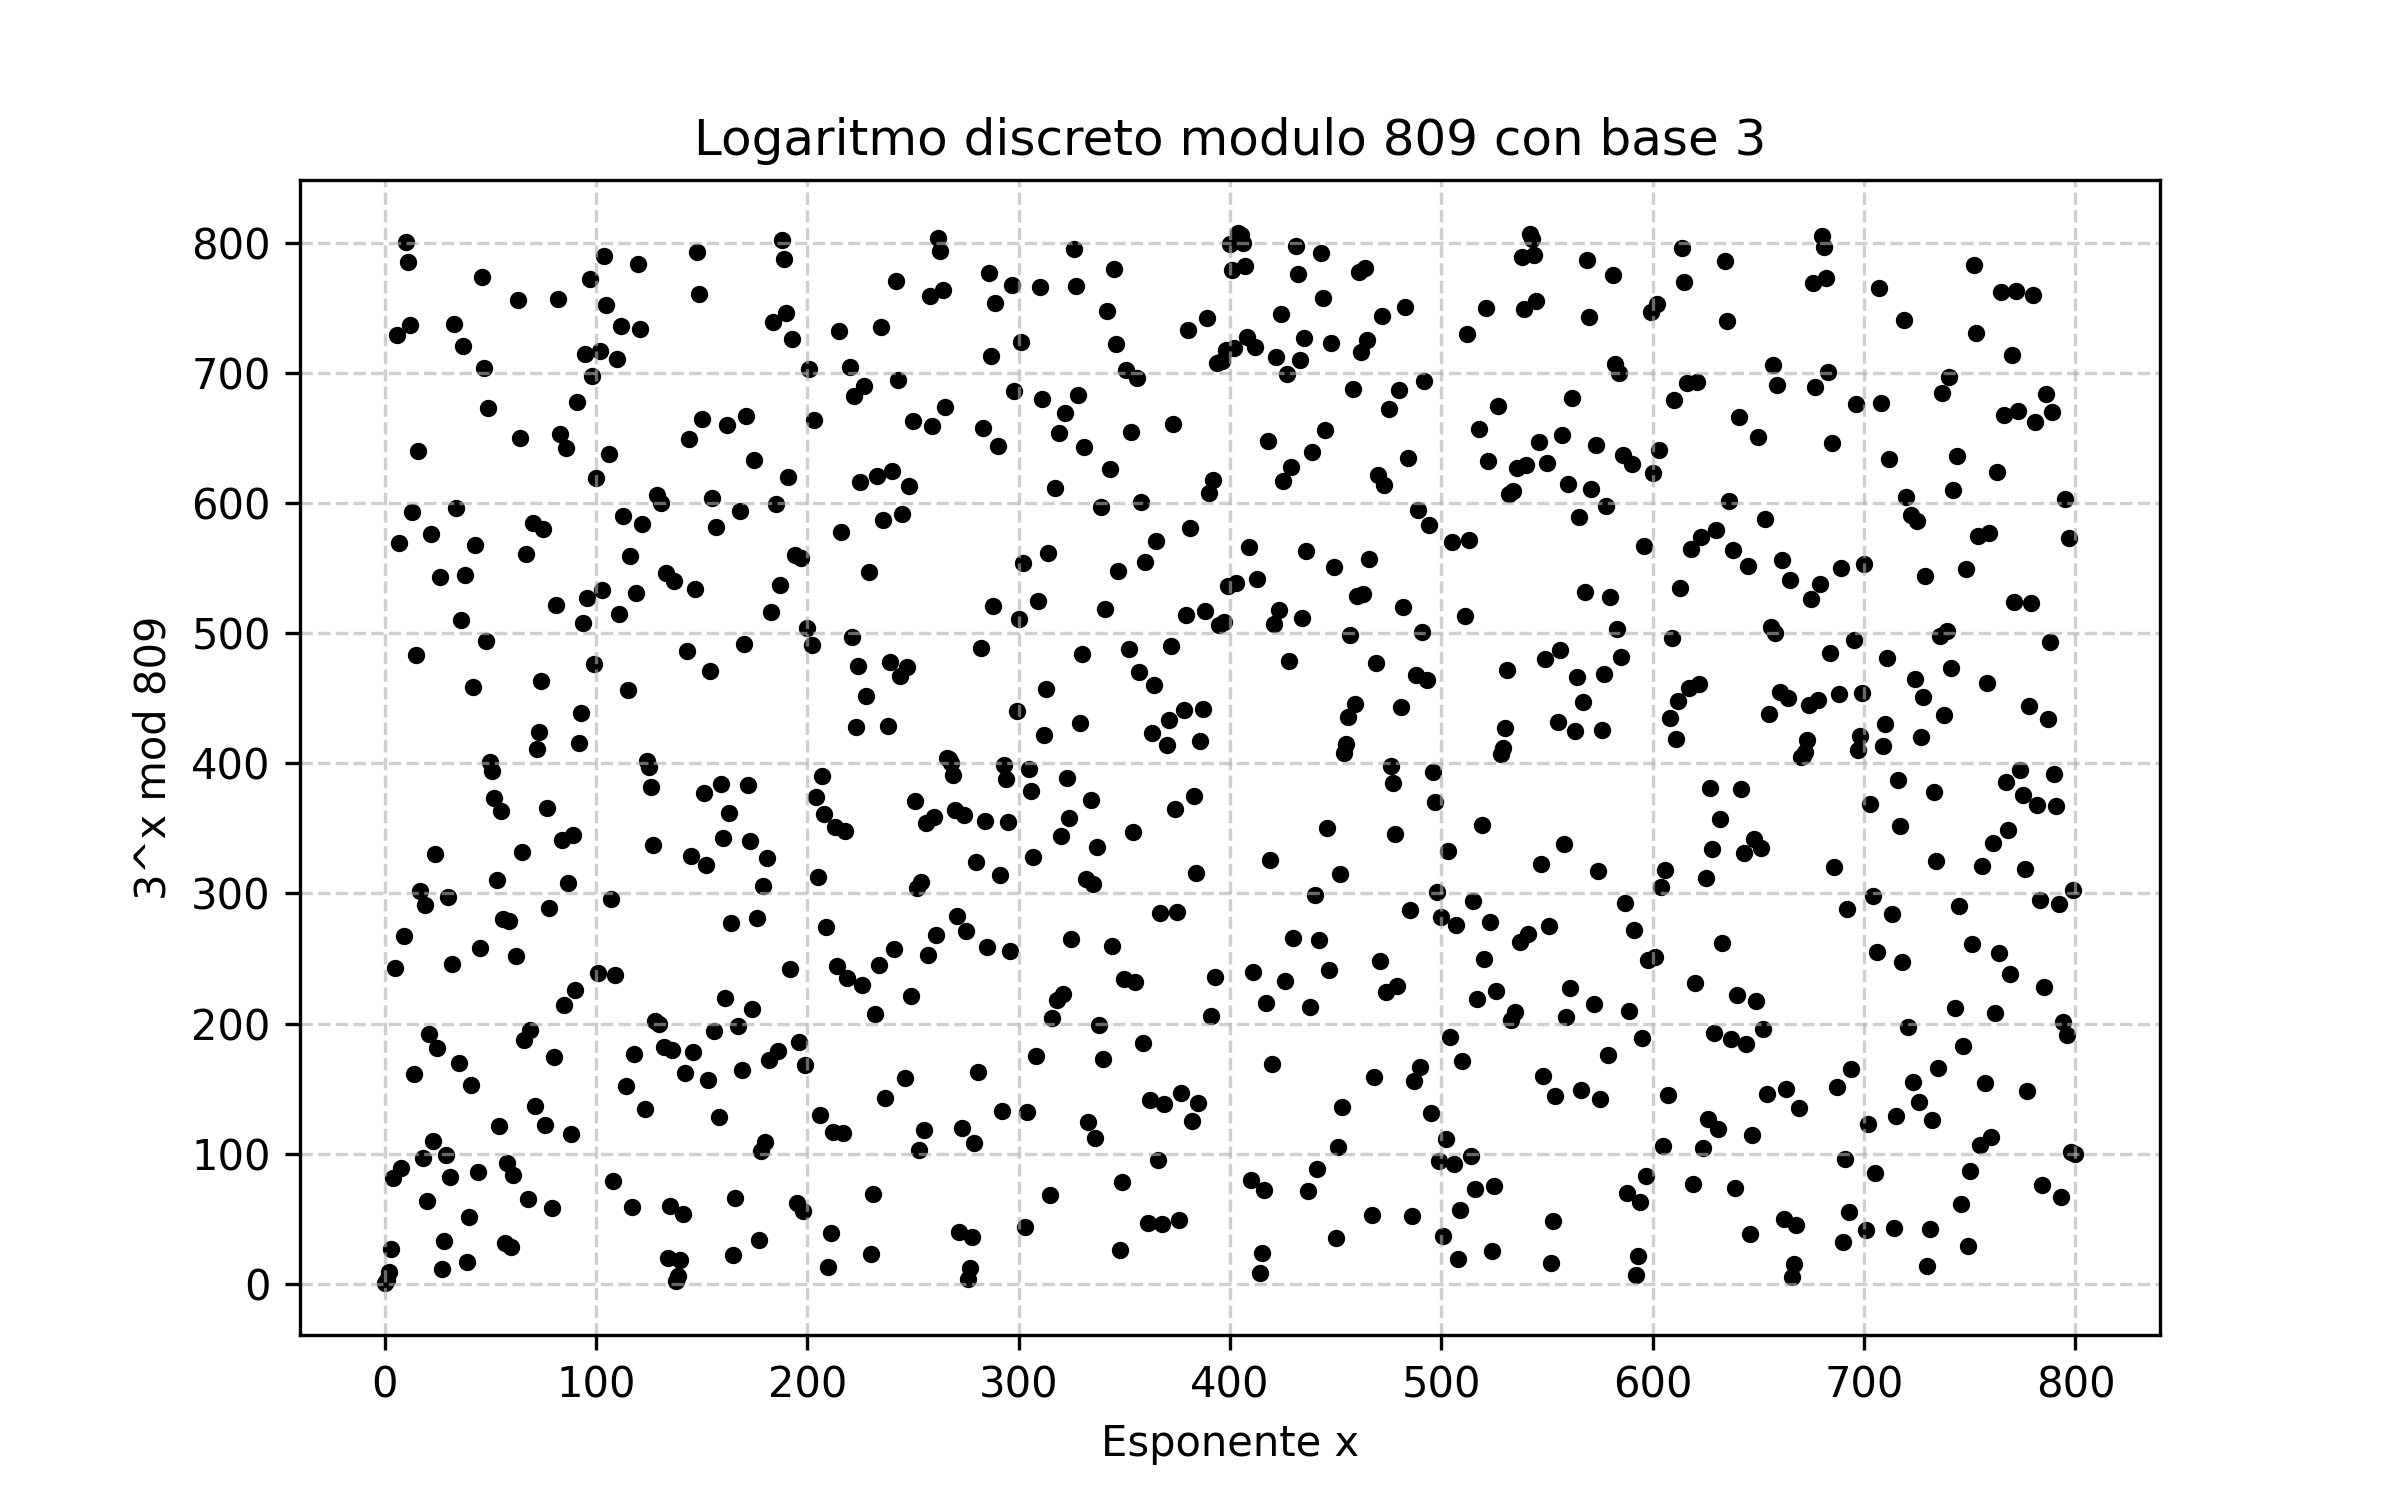
\includegraphics[width=\textwidth]{images/logaritmo_discreto.png}
    \caption{Grafico del logaritmo discreto.}
    \label{fig:discreto}
  \end{subfigure}
  \hfill
  \begin{subfigure}{0.48\textwidth}
    \centering
    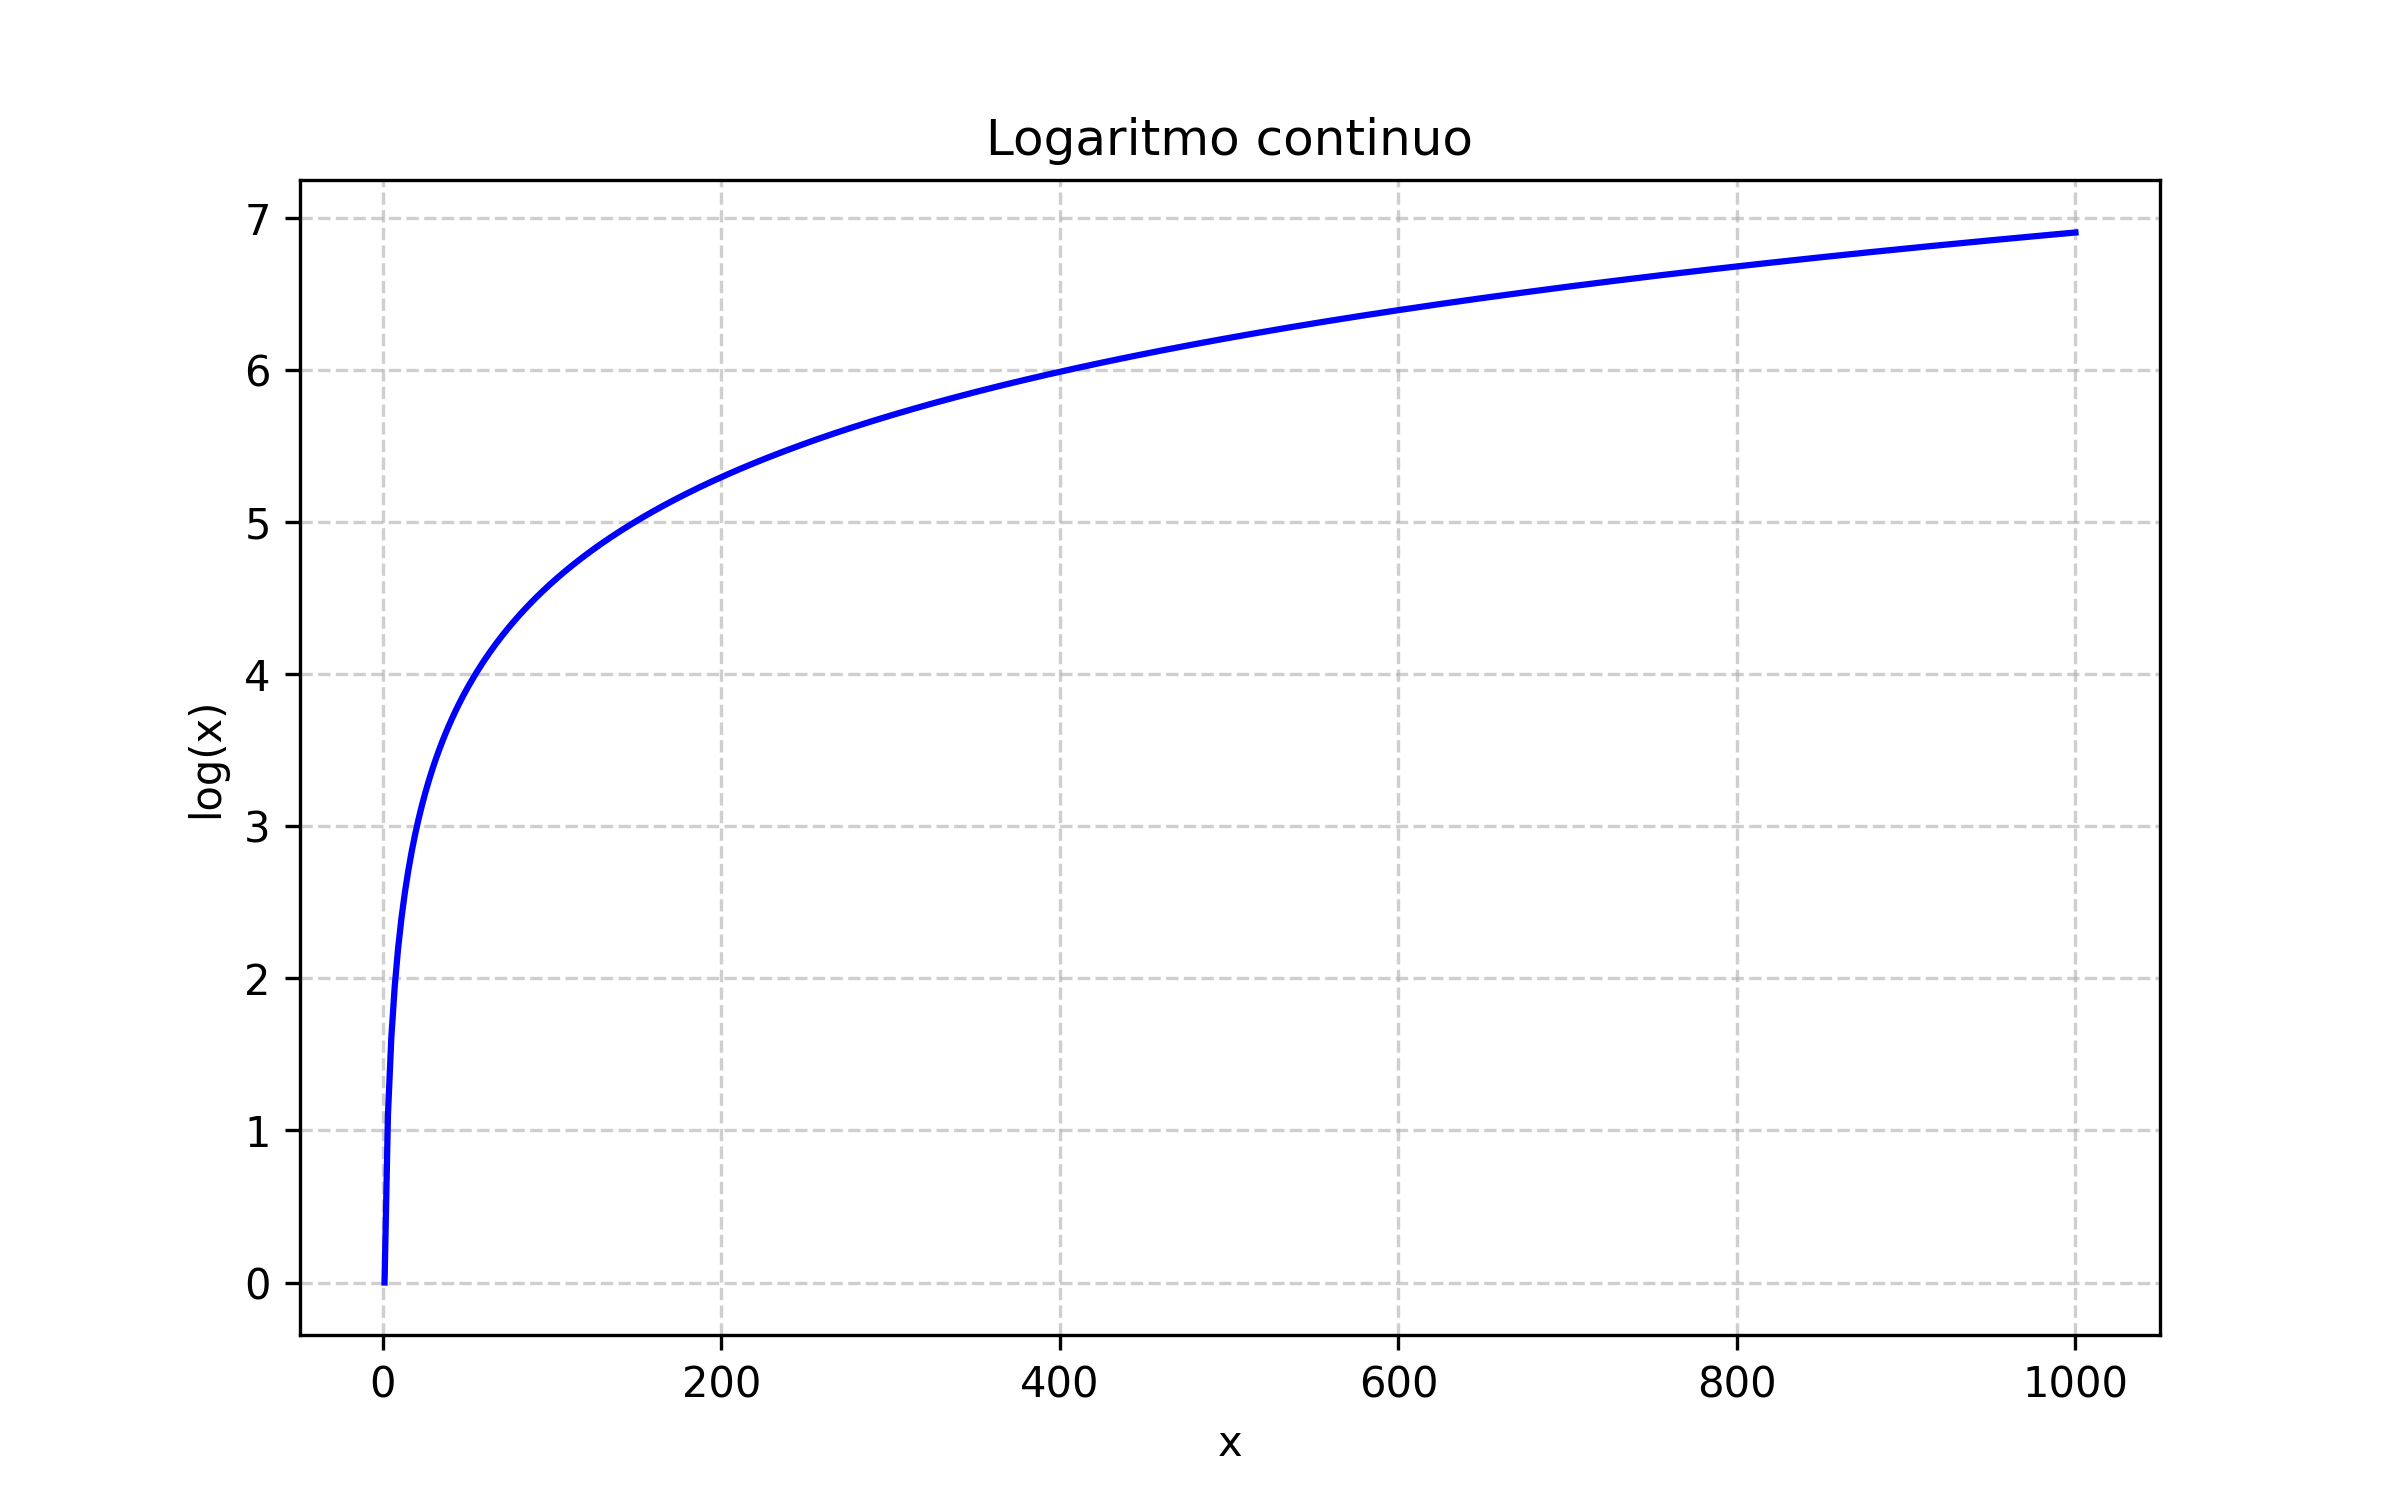
\includegraphics[width=\textwidth]{images/logaritmo_continuo.png}
    \caption{Grafico del logaritmo continuo.}
    \label{fig:continuo}
  \end{subfigure}
  \caption{Confronto tra logaritmo discreto e logaritmo continuo.}
  \label{fig:logaritmi}
\end{figure}

Il motivo principale per cui il logaritmo discreto risulta difficilmente calcolabile, a differenza del logaritmo continuo, risiede nella struttura discreta e ciclica del gruppo modulare.
Come mostrato in \autoref{fig:discreto}, i punti ottenuti mediante l'esponenziazione modulare risultano distribuiti in maniera apparentemente casuale all'interno del piano cartesiano, senza seguire un andamento regolare o monotono.
La funzione esponenziale modulo $p$, infatti, non è monotona e presenta un comportamento periodico, il che rende impossibile definire un'inversa diretta e, di conseguenza, calcolare agevolmente il logaritmo discreto.

\section{AES-GCM}\label{sec:aes}

L'\textbf{AES (Advanced Encryption Standard)}, conosciuto anche come \textbf{Rijndael}, sviluppato da J. Daemen and V. Rijmen, il cui funzionamento è descritto nel libro \textit{The Design of Rijndael: AES - The Advanced Encryption Standard} \cite{book}, è un algoritmo di cifratura simmetrica a blocchi, standardizzato dal NIST (National Institute of Standards and Technology) nel 2001 per sostituire il precedente DES (Data Encryption Standard). È oggi uno degli algoritmi crittografici più utilizzati al mondo, grazie alla sua sicurezza e all’efficienza sia su hardware che su software

Rijndael è una rete a sostituzione e permutazione. È veloce sia se sviluppato in software sia se sviluppato in hardware, è relativamente semplice da implementare, richiede poca memoria e offre un buon livello di protezione, motivi che complessivamente l'hanno reso il preferito rispetto agli altri algoritmi proposti. Nell'AES il blocco è di dimensione fissa (128 bit) e la chiave può essere di 128, 192 o 256 bit.

L’\textbf{AES-GCM (Galois/Counter Mode)}, descritto nello standard RFC 5288 \textit{AES Galois Counter Mode
(GCM) Cipher Suites for TLS} \cite{rfc5288}, è una modalità di utilizzo di AES che fornisce cifratura autenticata.
Questo significa che garantisce sia confidenzialità, ossia i dati sono cifrati con AES in modalità CTR (Counter Mode), oltre a garantire integrità e autenticità, ovvero un tag di autenticazione assicura che i dati non siano stati alterati.
AES-GCM è oggi una delle modalità più diffuse, usata in protocolli come SSH, QUIC/HTTP3, e nel Wi-Fi moderno.

\section{SHA-256}\label{sec:sha}

Una \textbf{funzione di hash crittografica (CHF)} è un algoritmo che associa un input arbitrario a un output di lunghezza fissa $n$ bit, garantendo proprietà fondamentali per la sicurezza:

\begin{itemize}
    \item \textbf{Uniformità}: ogni valore di hash ha probabilità $2^{-n}$ di comparire.
    \item \textbf{Resistenza alla preimmagine}: dato un hash, è computazionalmente infattibile ricavare l'input corrispondente ($\approx 2^n$ tentativi).
    \item \textbf{Resistenza alla seconda preimmagine}: data una stringa, è difficile trovarne un'altra con lo stesso hash.
    \item \textbf{Resistenza alle collisioni}: è improbabile trovare due input distinti con lo stesso hash; la complessità attesa è $2^{n/2}$.
\end{itemize}

\texttt{SHA-256} (Secure Hash Algorithm 256-bit) \cite{FIPS180-4} è una funzione di hash crittografica appartenente alla famiglia \texttt{SHA-2}, progettata dalla National Security Agency (NSA) e pubblicata dal NIST nel 2001 come successore di \texttt{SHA-1}.

\texttt{SHA-256} produce un digest di 256 bit, ossia una stringa di 64 caratteri esadecimali, indipendentemente dalla dimensione del messaggio in ingresso. Questa proprietà consente di trattare l'hash come una sorta di "impronta digitale" univoca del dato, utile per verificarne l'integrità e l'autenticità senza dover conservare l'intero contenuto originale.

Dal punto di vista operativo, l'algoritmo segue una struttura tipica delle funzioni di hash della famiglia Merkle–Damgård: al messaggio viene aggiunto inizialmente del padding e suddiviso in blocchi di 512 bit, che vengono elaborati iterativamente da una funzione di compressione basata su operazioni bitwise, somme modulari e funzioni non lineari. Alla fine di questa elaborazione, lo stato interno dell'algoritmo viene trasformato nell'hash finale di 256 bit.

Grazie a questa costruzione, \texttt{SHA-256} è oggi uno degli algoritmi più utilizzati in ambito crittografico. Viene impiegato in protocolli come TLS e IPsec, nei sistemi di firma digitale come DSA ed ECDSA, oltre ad avere un ruolo cruciale nel funzionamento delle blockchain e dei sistemi di proof-of-work, dove garantisce l'imprevedibilità e la verificabilità delle operazioni.
\chapter{Schnorr: Identificazione e Firma Digitale}

In questo capitolo verranno presentati i protocolli di Zero-Knowledge Proof (ZKP), introdotti per la prima volta alla fine degli anni '80 da Shafi Goldwasser, Silvio Micali e Charles Rackoff nel documento \textit{The Knowledge Complexity of Interactive Proof-Systems}\cite{doi:10.1137/0218012}. Particolare attenzione sarà dedicata al \textbf{protocollo di identificazione di Schnorr} e al corrispondente \textbf{schema di firma digitale}.

\section{Protocolli "Zero Knowledge Proof"}\label{sec:zkp}

\begin{de}[Zero-Knowledge-Proof Protocol] 
	Un protocollo conosciuto nella crittografia come \textit{Zero-Knowledge-Proof Protocol} (indicato con ZK oppure ZKP) rappresenta uno schema di dimostrazione nel quale un soggetto, detto \textbf{Prover}, deve convincere un secondo soggetto, detto \textbf{Verifier}, che una \textbf{dichiarazione} chiamata è vera, senza dover offrire informazioni aggiuntive riguardo il\textbf{testimone segreto (Witness)} che la rende vera.
\end{de}

L'intuizione alla base della dimostrazione a conoscenza zero è che è banale convincere del possesso di informazioni sensibili semplicemente rivelandole, mentre risulta più complesso  dimostrare il possesso di tali informazioni senza dover rivelarle.

Le dimostrazioni a conoscenza zero possono essere interattive, infatti tra Prover e Verifier si crea una comunicazione nella quale si effettua uno scambio di messaggi secondo un protocollo ben determinato. Esistono anche dimostrazioni a conoscenza zero non interattive, nelle quali il Prover convince il Verifier inviando un solo messaggio.

Al fine di chiarire meglio il funzionamento dei protocolli ZKP, si consideri il seguente esempio astratto.

Si tratta di una storia che racchiude al meglio i principi fondamentali delle dimostrazioni a conoscenza zero. È stato presentato per la prima volta da Jean-Jacques Quisquater in \cite{10.1007/0-387-34805-0_60}.

L’esempio, noto come storia della caverna di Alì Babà, descrive una situazione in cui un Prover (Peggy) deve convincere un Verifier (Victor) di conoscere un segreto (la parola magica che apre una porta nella caverna), senza però rivelarlo direttamente.

In questa storia, Peggy, è in possesso della parola segreta in grado di aprire una porta magica in una caverna. La caverna è a forma di anello con l'ingresso da una parte e, dal lato opposto, la porta magica che impedisce il passaggio da un percorso all'altro come mostrato in \autoref{fig:ali_baba_cave}. Victor vuole sapere se Peggy conosce o meno la parola segreta ma Peggy essendo una persona riservata, non vuole rivelare a Victor la parola magica. I percorsi sono etichettati con A (sinistro) e B (destro). Victor aspetta all'entrata mentre Peggy sceglie quale percorso usare senza che Victor lo sappia. Dopodiché, Victor entra nella caverna e grida quale percorso - scelto a caso - deve usare Peggy per fare ritorno all'entrata. A patto che conosca davvero la parola magica, sarebbe facile: aprirebbe la porta, se necessario, per tornare indietro seguendo il percorso desiderato.

% TODO: MODIFICARE LA CITAZIONE

Tuttuvia, supponendo che Peggy non conosca la parola magica, avrebbe potuto fare ritorno usando il percorso indicato solo se Victor avesse scelto il percorso seguito inizialmente da Peggy. Siccome Victor sceglie casualmente il percorso, lei ha il $50\%$ di probabilità di indovinare correttamente il percorso da seguire per fare ritorno. Se questo processo viene ripetuto, diciamo, 20 volte, allora la probabilità di successo, ovvero di anticipare correttamente la richiesta di Victor, si ridurrebbe a $\frac{1}{2^{20}}$.

In conclusione, se Peggy ripetutamente appare all'entrata seguendo il percorso scelto da Victor, allora si può concludere che Peggy conosce la parola magica.

\begin{figure}[h!]
	\centering
	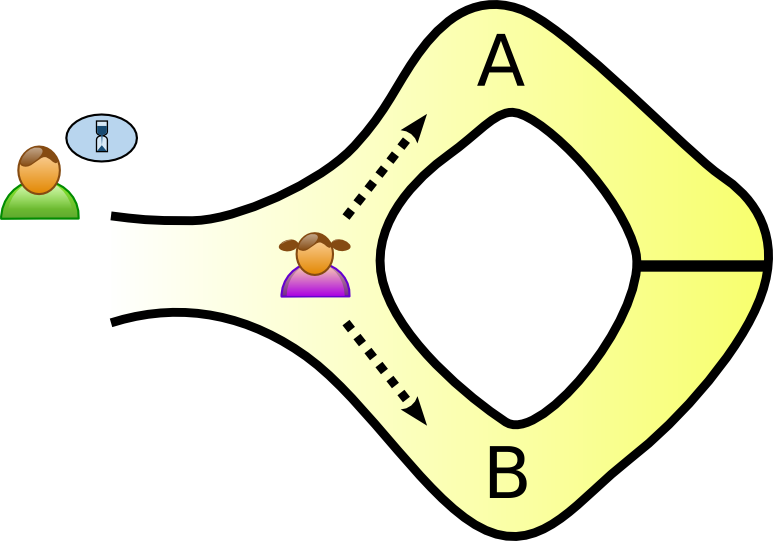
\includegraphics[width=0.6\textwidth]{images/ali_baba_cave.png}
	\caption{Rappresentazione della caverna di Alì Babà.}
	\label{fig:ali_baba_cave}
\end{figure}

Ora che è stato chiarito meglio il funzionamento dei protocolli ZKP, si piò procedere con elencare le tre proprietà che una dimostrazione ZKP deve soddisfare.

\subsection{Proprietà}\label{sec:zkp-prop}

\begin{enumerate}
	\item \textbf{Completezza}: Se l'affermazione è vera, allora un verificatore onesto sarà convinto di questo fatto da un dimostratore onesto.
	\item \textbf{Correttezza}: Se l'affermazione è falsa, allora nessun dimostratore può imbrogliare un verificatore onesto che il fatto è vero, o meglio la probabilità di riuscire a convincerlo può essere ridotta a piacimento.
	\item \textbf{Zero Knowledge Proof}: Se l'affermazione è vera, allora nessun verificatore è in grado di acquisire informazioni aggiuntive oltre al fatto che l'affermazione è vera. 
\end{enumerate}

La ricerca nell'ambito dei protocolli ZKP ha portato allo sviluppo di sistemi di autenticazione a conoscenza zero, in cui un'entità prova a dimostrare la propria identità ad un'altra entità tramite un'informazione segreta (es. password) senza rivelare tale informazione. Questo tipo di autenticazione è chiamato "Zero Knowledge - Proof of Knowledge" (prova di conoscenza a conoscenza zero).

Per implementare tali protocolli in modo efficiente e sicuro sono stati sviluppati diversi schemi formali. Tra i più studiati e applicati troviamo i cosiddetti \textit{$\Sigma$-Protocols}\footnote{Il protocollo d'identificazione di Schnorr è un caso speciale di Sigma Protocol ed è oggetto di studio di questa tesi.}, che costituiscono una classe di protocolli interattivi a tre mosse (commitment, challenge, response) particolarmente adatti alla costruzione di prove di conoscenza a conoscenza zero. 

\newpage

\section{Protocolli Sigma}

In questa sezione si andrà a discutere dei protocolli $\Sigma$\footnote{Letto \textit{Sigma}, dove la prima parte richiama lo "zig-zag" delle tre mosse tipiche di un protocollo interattivo, mentre il suffisso è un'abbreviazione di "Merlin-Artur".} introdotti per la prima volta da R. Cramer nella sua tesi di dottorato \cite{pub:21438}. In particolare verrà data una definizione di cos'è un protocollo Sigma, di come funziona e quali sono le proprietà fondamentali. L'argomento è trattato con maggiori dettagli nel libro D. Boneh and V. Shoup, \textit{A Graduate Course in Applied Cryptography}, Cap. 19.4 \cite{boneh2020applied}.

\begin{de}[Relazione Effettiva] Una \textbf{relazione effettiva} è una relazione binaria $\mathcal{R} \subseteq \mathcal{X} \times \mathcal{Y}$, dove $\mathcal{X},\ \mathcal{Y} \text{ e } \mathcal{R}$ sono degli insiemi finiti riconoscibili in modo efficiente. Gli elementi di $\mathcal{Y}$ sono detti \textbf{affermazioni (statements)}. Se $(x, y) \in \mathcal{R}$, allora $x$ è detto \textbf{testimone per (witness for)} $y$.
\end{de}

\begin{de}[Protocollo Sigma]\label{def:sigma} Sia $\mathcal{R} \subseteq \mathcal{X} \times \mathcal{Y}$ una relazione effettiva. Un \textbf{Protocollo Sigma} su $\mathcal{R}$ è una coppia $(P, V)$.
	\begin{itemize}[itemsep=0.3em, topsep=0.2em]
		\item $P$ è un protocollo interattivo chiamato \textbf{prover}, e prende in input una coppia \textit{testimone-affermazione} $(x, y) \in \mathcal{R}$.
		\item $V$ è un protocollo interattivo chiamato \textbf{verifier}, prende in input un'\textit{affermazione} $y \in \mathcal{Y}$ ($V$ non è a conoscenze del testimone $x$), e restituisce in output \textit{accetta} o \textit{rigetta}.
		\item $P$ e $V$ sono strutturati in modo che un'interazione tra loro avvenga nel seguente modo (vedere \autoref{fig:sigma-protocol}):
		      \begin{itemize}[itemsep=0.1em, topsep=0.2em]
		      	\item Per iniziare, $P$ computa un messaggio $t$, chiamato \textbf{commitment}, e lo invia a $V$.
		      	\item Una volta ricevuto il messaggio $t$ da $P$, $V$ sceglie casualmente un valore $c$, chiamato \textbf{challenge}, da uno spazio finito $\mathcal{C}$, detto \textbf{challenge space}, e lo invia a $P$.
		      	\item Una volta ricevuta la challenge $c$ da $V$, $P$ computa  $z$, detto \textbf{response}, e lo invia a $V$.
		      	\item Ricevuto $z$, $V$ decide se \textit{accettare} o \textit{rigettare} dopo aver calcolato una funzione dipendente dall'affermazione $y$ e dalla conversazione (\textbf{conversation}) $(t, c, z)$.
		      	              
		      	      In particolare, $V$ non effettua ulteriori scelte casuali se non per scegliere $c$, il resto delle computazioni sono strettamente \textit{deterministiche}. 
		      \end{itemize}
	\end{itemize}
\end{de}

\newpage

\begin{figure}[h!]
	\centering
	\begin{tikzpicture}[>=latex, font=\small]
		
		\node (P) at (-3,0) {$\underline{P(x, y)}$};
		\node (V) at (4,0) {$\underline{V(y)}$};
		
		\node[left] at (-3,-1) {\textit{commitment} $t$};
		\draw[->] (-3,-1.3) -- (4,-1.3) node[midway,above] {$t$};
		
		\node[right] at (4,-2) {\textit{challenge}: $c \;\overset{R}{\leftarrow}\; \mathcal{C}$};
		
		\draw[<-] (-3,-2.3) -- (4,-2.3) node[midway,below] {$c$};
		
		\node[left] at (-3,-3) {\textit{response} $z$};
		\draw[->] (-3,-3.3) -- (4,-3.3) node[midway,above] {$z$};
		
		\node[right] at (4,-3.6) {\textit{accetta/rigetta}};
		
	\end{tikzpicture}
	\caption{Schema di un protocollo $\Sigma$ interattivo}
	\label{fig:sigma-protocol}
\end{figure}
\hrulefill

Come specificato nella \autoref{def:sigma}, è richiesto che il verifier calcoli una funzione 
$$f :  (y, t, c, z) \to \{\textit{accetta}, \textit{rigetta}\},$$
dipendente da $y$ e dalla conversazione $(t, c, z)$.
Se l'esisto della funzione è \textit{accetta}, allora la conversazione $(t, c, z)$ è detta \textbf{accettata per} $y$.

È chiaro che un'interazione tra un verifier e un prover \textit{onesto} porti sempre ad una conversazione accetata. Conversazioni rigettate si verificano, ad esempio, quando il verifier interagisce con un prover \textit{disonesto} che non rispetta il protocollo concordato.

Inoltre, in molte applicazioni dei protocolli Sigma è richiesto che lo spazio delle challenge $\mathcal{C}$ sia super-poly\footnote{Nella teoria della complessità, quando si parla di \textbf{super-poly space} si intende uno spazio di memoria che cresce più velocemente di qualunque polinomio nella dimensione dell'input.}.

\subsection{Proprietà}\label{sec:sigma-prop}

I protocolli $\Sigma$ si inseriscono nella categoria dei Zero-Knowledge-Proof e, di conseguenza, rispettano tutte e tre le proprietà fondamentali già elencate nella \autoref{sec:zkp-prop}. Tuttavia, queste vengono formulate in maniera più specifica, dando origine alle nozioni di \textbf{perfect completeness}, \textbf{special soundness} e \textbf{special honest-verifier zero-knowledge (HVZK)}.

\begin{itemize}
	\item \textbf{Perfect Completeness}: $\forall (x, y) \in \mathcal{R}$, quando $P(x, y)$ e $V(y)$ interagiscono tra loro, $V(y)$ deve \textit{accettare} sempre. Formalmente, abbiamo che:
	      $$\forall (x, y) \in \mathcal{R},\ \Pr \left[\langle P(x, y), V(y) \rangle =\ accetta \right] = 1$$
	      dove $\langle P(x, y), V(y) \rangle$ rappresenta l'interazione tra $V$ e $P$.
	\item \textbf{Special Soundness}: Sia $(P, V)$ un protocollo Sigma per la relazione $\mathcal{R} \subseteq \mathcal{X} \times \mathcal{Y}$. Si dice che $(P, V)$ offre una solidità speciale (\textbf{special soundness}) se esiste un algoritmo deterministico efficiente \textit{Ext}, chiamato estrattore di testimoni (\textbf{witness extractor}), avente la seguente proprietà: ogni volta che ad \textit{Ext} viene fornito in input un'affermazione $y \in \mathcal{Y}$ e due conversazioni di accettazione $(t, c, z)$ e $(t, c', z')$, con $c \neq c'$, l'algoritmo restituisce sempre in output $x \in \mathcal{X}$ tale che $(x, y) \in \mathcal{R}$, dove $x$ è il testimone di $y$.
	\item \textbf{Special HVZK}: Sia $(P, V)$ un protocollo Sigma per la relazione $\mathcal{R} \subseteq \mathcal{X} \times \mathcal{Y}$ con spazio delle sfide $\mathcal{C}$. Si dice che $(P, V)$ è un verificatore onesto a conoscenza zero (\textbf{special HVZK}), se esiste un algoritmo probabilistico efficiente \textit{Sim}, chiamato \textbf{simulatore}, che prende in input $(y, c) \in \mathcal{Y} \times \mathcal{C}$ avente le seguenti proprietà:
	      \begin{enumerate}
	      	\item Per ogni input $(y, c) \in \mathcal{Y} \times \mathcal{C}$, l'algoritmo \textit{Sim} produce in output una coppia $(t, z)$ tale che $(t, c, z)$ è una conversazione accettata per $y$.
	      	\item Per ogni $(x, y) \in \mathcal{R}$, se si calcola
	      	      $$c \overset{R}{\leftarrow} \mathcal{C},\ (t, z) \overset{R}{\leftarrow} Sim(y, c),$$
	      	      allora $(t, c, z)$ ha la stessa distribuzione di quella di una trascrizione di una conversazione tra $P(x, y)$ e $V(y)$.
	      	      
	      	      In altre parole, questa proprietà dice che, dato un protocollo Sigma $(P, V)$ per $\mathcal{R} \subseteq \mathcal{X} \times \mathcal{Y}$ e sia la coppia $(x, y) \in \mathcal{R}$, una conversazione tra $P(x, y)$ e $V(y)$ non rivela alcuna informazione aggiuntiva riguardo al testimone $x$.
	      \end{enumerate}
\end{itemize}

A primo impatto, sembrerebbe che la \textbf{special soundness} sia una proprietà indesiderabile: Perché vorremmo una proprietà che ci permette di estrarre il testimone $x$, date due conversazioni accettate?
Innanzitutto, è importante osservare che la definizione vale soltanto se le due conversazioni condividono lo stesso \textit{commitment} $t$ mentre le \textit{challenge} $c$ sono diverse. Infatti, possiamo dire che \textit{se qualcuno riesce a rispondere correttamente a due sfide diverse partendo dallo stesso $t$, allora deve "sapere qualcosa di vero" sul segreto}. Se $t$ fosse diverso, non avrebbe senso dire che "due risposte diverse rivelano il segreto": sarebbero due protocolli indipendenti. Inoltre, poiché $t$ viene scelto in modo casuale dal Prover, è improbabile che un \textit{honest Prover} invii due volte lo stesso $t$.
Quindi, il caso in cui il Verifier ottiene due conversazioni con lo stesso $t$ ma sfide diverse accade solo se il Prover è sotto il controllo dell'estrattore (come avviene nella definizione teorica di soundness).

In particolare, la \textbf{special soundness}, ci garantisce:
\begin{itemize}
    \item \textbf{Soundness}: Significa che un Prover che non conosce $x$ non può rispondere correttamente a più di una sfida, perché altrimenti sarebbe possibile estrarre $x$ dalle sue risposte.
    Di conseguenza, un truffatore che vuole ingannare il Verifier ha una probabilità di successo al massimo pari a: \[\frac{1}{|\mathcal{C}|}\].
    \item \textbf{Proof of Knowledge}: Consente di costruire un estrattore \textit{Ext}: un algoritmo che, interagendo con un Prover qualunque, può "riavvolgerlo" allo stato precedente alla ricezione della challenge $c$ (mantenendo lo stesso commitment $t$) e ottenere due conversazioni valide per estrarre il segreto $x$. Questo serve a formalizzare che il protocollo non dimostra solo che "l'affermazione è vera", ma che il Prover conosce effettivamente il testimone $x$. Se il Prover fosse uno non onesto, allora non sarebbe possibile generare due conversazioni valide "riavvolgendolo", in quanto per ipotesi, non conosce il testimone $x$.
\end{itemize}

\newpage

\section{Firme Digitali}\label{sec:sig-dig}

Una \textbf{firma digitale} è un meccanismo crittografico che permette di garantire \textbf{l'autenticità}, \textbf{l'integrità} e \textbf{la non ripudiabilità} di un documento o di un messaggio elettronico. Nello specifico, si vuole assicurare che un'informazione:
\begin{itemize}
    \item Provenga davvero dal mittente dichiarato (autenticità).
    \item Non sia stata alterata durante la trasmissione o l'archiviazione (integrità).
    \item Non possa essere negata dal mittente (non ripudiabilità).
\end{itemize}

Dal punto di vista tecnico, la firma digitale si basa sulla crittografia asimmetrica: ogni utente possiede una coppia di chiavi, una privata e una pubblica. La chiave pubblica viene utilizzata per generare la firma sul documento mentre la chiave privata viene usata dai destinatari per verificarne la validità. In pratica, il documento/messaggio non viene firmato direttamente, ma se ne calcola un hash. Questo hash viene poi cifrato con la chiave privata del mittente: il risultato è la firma digitale. Chi riceve il documento potrà ricalcolare l'hash e confrontarlo con quello decifrato usando la chiave pubblica del mittente: se coincidono, la firma è valida.

Le firme digitali sono oggi fondamentali in moltissimi contesti: posta elettronica certificata, documenti legali, contratti online, servizi bancari, e in generale in ogni scenario in cui sia necessario garantire sicurezza e fiducia nello scambio di informazioni.

Di seguito, una definizione formale di firma digitale ripresa da (D. Boneh and V. Shoup, \textit{A Graduate Course in Applied Cryptography}, Cap. 13.1 Pag 528 \cite{boneh2020applied}).
\begin{de}[Firma digitale]
    Un \textbf{sistema di firme digitali} $\mathcal{S} = (G,\ S,\ V)$ è una tripla di algoritmi efficienti, $G,\ S,\ V$, dove $G$ è chiamato \textbf{algoritmo di generazione delle chiavi}, $S$ è chiamato $\textbf{algoritmo di firma}$ e, infine, $V$ è detto \textbf{algoritmo di verifica}. Dunque, $S$ è usato per \textit{generare} le firme e $V$ è usato per \textit{verificare} le firme.
    Nello specifico,
    \begin{itemize}
        \item $G$ è un algoritmo \textit{probabilistico} che non richiede nessun input. Fornisce invece in output una coppia $(pk, sk)$, dove $sk$ è la \textbf{chiave segreta di firma} e $pk$ è la \textbf{chiave pubblica di verifica}.
        \item $S$ è anch'esso un algoritmo \textit{probabilistico} che ha il ruolo di computare 
        \[\sigma \overset{R}{\leftarrow} S(sk,\ m),\]
        dove $sk$ è la chiave segreta generata da $G$ ed $m$ è il messaggio. L'algoritmo restituisce in output la \textbf{firma} $\sigma$.
        \item $V$ è un algoritmo \textit{deterministico}, tale che 
        \[\texttt{accept or reject} \leftarrow V(pk,\ m,\ \sigma).\]
        \item È inoltre richiesto che la firma generata da $S$ sia sempre accettata da $V$. Ovvero, per ogni coppia $(pk. sk)$ generata da $G$ e per ogni messaggio $m$, si ha:
        \[\text{Pr}[V(pk,\ m,\ S(sk,\ m)) = \texttt{accept}] = 1.\]
    \end{itemize}
    Infine, diremo che i messaggi $m$ risiedono in uno \textbf{spazio di messaggi} finito $\mathcal{M}$ e le firme risiedono in uno \textbf{spazio di firme} finito $\Sigma$. Diremo inoltre che $\mathcal{S} = (G,\ S,\ V)$ è definito su $(\mathcal{M},\ \Sigma)$.
\end{de}

\subsection{Euristica di Fiat-Shamir per le Firme}\label{sec:fiat-shamir}

È possibile convertire protocolli Sigma in schemi di firma digitale usando una tecnica sviluppata da Fiat e Shamir conosciuta come \textbf{l'euristica di Fiat-Shamir} oppure come la \textbf{trasformazione di Fiat-Shamir} \cite{10.1007/3-540-47721-7_12}. Gli elementi costitutivi sono i seguenti:

\begin{itemize}
    \item Un protocollo Sigma $(P,\ V)$ definito per una relazione $\mathcal{R} \subseteq \mathcal{X} \times \mathcal{Y}$; assumiamo inoltre che le conversazioni siano della forma $(t,\ c,\ z)$, dove $t \in \mathcal{T},\ c \in \mathcal{C},\ z \in \mathcal{Z}$;
    \item Un algoritmo di generazione delle chiavi $G$ per $\mathcal{R}$;
    \item Una funzione hash $H: \mathcal{M} \times \mathcal{T} \rightarrow \mathcal{C}$, modellata come un'oracolo casuale; l'insieme $\mathcal{M}$ è lo spazio dei messaggi per lo schema di firme digitali.
\end{itemize}

Lo schema di firme di Fiat-Shamir derivato da $G$ e dal protocollo Sigma $(P, V)$ funziona nel seguente modo:

\begin{itemize}
    \item L'algoritmo di generazione delle chiavi è $G$, dunque, una chiave pubblica è della forma $pk = y$, dove $y \in \mathcal{Y}$ e una chiave segreta è della forma $sk = x$, dove $(x, y) \in \mathcal{R}$.
    \item Affinché possa firmare un messaggio $m \in \mathcal{M}$ usando una chiave segreta $sk = (x, y)$, l'algoritmo di firma deve funzionare nel seguente modo:
    \begin{itemize}
        \item Inizializza il prover $P(x, y)$, ottenendo il \textit{commitment} $t \in \mathcal{T}$;
        \item Calcola la \textit{challenge} $c \leftarrow H(m, t)$;
        \item Infine, immette $c$ nel prover, ottenendo una \textit{response} $z$ e restituendo in output la firma $\sigma := (t, z) \in \mathcal{T} \times \mathcal{Z}$. 
    \end{itemize}
    \item Per verificare la firma $\sigma = (t, z) \in \mathcal{T} \times \mathcal{Z}$ su un messaggio $m \in \mathcal{M}$ usando la chiave pubblica $pk = y$, l'algoritmo di verifica calcola $c \leftarrow H(m, t)$ e verifica che $(t, c, z)$ è una conversazione accettata per $y$.
\end{itemize}

\section{Protocollo d'Identificazione di Schnorr}\label{sec:schnorr}

Il paragrafo che segue è dedicato all'argomento principale di questa tesi: il \textbf{protocollo d'identificazione di Schnorr}, ideato da Claus Peter Schnorr alla fine degli anni '80 nel documento \textit{Efficient signature generation by smart cards}\cite{Schnorr2005}. È uno dei più celebri esempi di Sigma protocol basato sul problema del logaritmo discreto. La sua importanza risiede nel fatto che fornisce una base per numerosi schemi di autenticazione moderni e di firme digitali (\textbf{firma digitale di Schnorr}).

La struttura del protocollo segue il paradigma \textbf{commitment-challenge-response}, tipico dei Sigma protocol, rispettando tutte le proprietà fondamentali: \textbf{perfect completeness, special soundness, special HVZK}.

\begin{de}
	Sia $\mathbb{G}$ un gruppo ciclico di ordine primo $q$ con generatore $g \in \mathbb{G}$ e sia $\mathcal{C} \subseteq \mathbb{Z}_q$. Il protocollo d'identificazione di Schnorr è identificato dalla tripla $\mathcal{I}_{sch} = (G, P, V)$, dove:
	\begin{itemize}
		\item $G$ rappresenta l'algoritmo di generazione delle chiavi e funziona nel seguente modo:
		      $$\alpha \overset{R}{\leftarrow} \mathbb{Z}_q,\ u \leftarrow g^{\alpha}$$
		      La chiave di verifica è $vk := u$, mentre la chiave segreta $sk := \alpha$.
		\item $P$ è il prover inizializzato con $sk = \alpha$ mentre $V$ è il verifier inizializzato con $vk = u$. Il protocollo di comunicazione tra $P$ e $V$ è il seguente, come mostrato in \autoref{fig:schnorr-protocol}:
		      \begin{enumerate}
		      	\item $P$ calcola $\alpha_t \overset{R}{\leftarrow} \mathbb{Z}_q$, $u_t \leftarrow g^{\alpha_t}$, e invia $u_t$ a $V$;
		      	\item $V$ calcola $c \overset{R}{\leftarrow} \mathcal{C}$, e lo invia a $P$;
		      	\item $P$ calcola $\alpha_z \leftarrow \alpha_t + \alpha c \in \mathbb{Z}_q$, inviandolo poi a $V$;
		      	\item $V$ effettua il seguente controllo: $$g^{\alpha_z} = u_t \cdot u^c$$ Se l'uguaglianza è verificata allora $V$ \textit{accetta}, altrimenti \textit{rigetta}. 
		      \end{enumerate}
	\end{itemize}
\end{de}

L'interazione tra $P(\alpha)$ e $V(u)$ genera una conversazione $(u_t, c, \alpha_z) \in \mathbb{G} \times \mathcal{C} \times \mathbb{Z}_q$. Tale conversazione è detta \textbf{di accettazione per} $u$ se il controllo che $V$ effettua è vero, ovvero se vale questa uguaglianza $g^{\alpha_z} = u_t \cdot u^c$. È di facile dimostrazione che qualsiasi interazione tra $P(\alpha)$ e $V(u)$ genera sempre una conversazione di accettazione, infatti, sapendo che $u_t = g^{\alpha_t}$ e $\alpha_z = \alpha_t + \alpha c$, allora
\begin{silentproof}
	\[
		g^{\alpha_z} = g^{\alpha_t + \alpha c} = g^{\alpha_t} \cdot g^{\alpha c} = u_t \cdot u^c
	\]
\end{silentproof}

\newpage

\begin{figure}[h!]
	\centering
	\begin{tikzpicture}[>=latex, font=\small]
		
		\node (P) at (-3,0) {$\underline{P(\alpha)}$};
		\node (V) at (3,0) {$\underline{V(u)}$};
		
		\node[left] at (-3,-1) {$\alpha_t \overset{R}{\leftarrow} \mathbb{Z}_q$, $u_t \leftarrow g^{\alpha_t}$};
		\draw[->] (-3,-1.3) -- (3,-1.3) node[midway,above] {$u_t$};
		
		\node[right] at (3,-2) {$c \;\overset{R} {\leftarrow}\; \mathcal{C}$};
		
		\draw[<-] (-3,-2.3) -- (3,-2.3) node[midway,below] {$c$};
		
		\node[left] at (-3,-3) {$\alpha_z \leftarrow \alpha_t + \alpha c \in \mathbb{Z}_q$};
		\draw[->] (-3,-3.3) -- (3,-3.3) node[midway,above] {$z$};
		
		\node[right] at (3,-3.6) {$g^{\alpha_z} \overset{?}{=} u_t \cdot u^c$};
		
	\end{tikzpicture}
	\caption{Interazione tra $P$ e $V$ nel Protocollo d'identificazione di Schnorr}
	\label{fig:schnorr-protocol}
\end{figure}
\hrulefill

\subsection{Proprietà}

Una volta chiarito il funzionamento del protocollo d'identificazione di Schnorr, occorre passare alla fase successiva, cioè fornire una dimostrazione della sua sicurezza. Il primo teorema enunciato di seguito dimostra che il protocollo è sicuro contro gli attacchi diretti (enumerazione). La dimostrazione di tale teorema si trova a Pag. 757 del libro Boneh and V. Shoup, \textit{A Graduate Course in Applied Cryptography} \cite{boneh2020applied}.

\begin{theorem}
	Assumendo che il problema del logaritmo discreto è difficile per il gruppo $\mathbb{G}$ e assumendo inoltre che $N := |\mathcal{C}|$ è super-poly, il protocollo d'identificazione di Schnorr è sicuro contro gli attacchi diretti.
\end{theorem}

Dal momento che il protocollo d'identificazione di Schnorr rientra nella classe dei $\Sigma$-Protocol, esso soddisfa per costruzione tutte le proprietà fondamentali descritte nella \autoref{sec:sigma-prop}. Nei paragrafi successivi mostreremo in dettaglio come ciascuna di queste proprietà risulti effettivamente rispettata, iniziando dall’analisi della proprietà di \textbf{special HVZK}.

\begin{theorem}\label{thm:schnorr-hvzk}
	Il protocollo d'identificazione di Schnorr è HVZK.
	\begin{proof}
		L'idea è di generare una conversazione simulata $(u_t, c, \alpha_z)$ definendo un simulatore \textit{Sim} con input $vk = u$ che generi questi messaggi nell'ordine \textit{inverso}. Il simulatore opera nel seguente modo, calcolando:
		\[
			\alpha_z \overset{R}{\leftarrow} \mathbb{Z}_q,\ c \overset{R}{\leftarrow} \mathcal{C},\ u_t \leftarrow g^{\alpha_z}\cdot u^{-c},
		\]
		producendo quindi in output la conversazione $(u_t, c, \alpha_z)$.
		        
		Rimane da dimostrare che l'output di \textit{Sim} abbia la stessa distribuzione di una comunicazione reale tra un prover $P$ e un verifier $V$. L'osservazione chiave, infatti, è che in un'interazione reale $c$ e $\alpha_z$ sono indipendenti, ovvero $c$ è distribuito uniformemente in $\mathcal{C}$ ed $\alpha_z$ è distribuito  uniformemente in $\mathbb{Z}_q$.
		        
		Inoltre, dati $c$ e $\alpha_z$, il prover $P$ calcola il valore $u_t$ determinato univocamente dall'equazione 
		\[
			g^{\alpha_z} = u_t \cdot u^c \Longleftrightarrow u_t = g^{\alpha_z}\cdot u^{-c}
		\]
		che è esattamente la regola con cui \textit{Sim} calcola $u_t$. Dunque, la distribuzione di $(u_t, c, \alpha_z)$ prodotta da \textit{Sim} coincide \textit{esattamente} con quella di una conversazione reale tra un prover $P$ e un verifier $V$. 
	\end{proof}
\end{theorem}


\begin{proposition}
	Il protocollo di Schnorr è anche \textbf{special HVZK}.
	\begin{proof}
		Dato in input $u \in \mathbb{G}$ e $c \in \mathcal{C}$, il simulatore può
		scegliere $\alpha_z \overset{R}{\leftarrow} \mathbb{Z}_q$ e calcolare
		\[
			u_t \leftarrow g^{\alpha_z} \cdot u^{-c}.
		\]
		L’argomento sulla distribuzione rimane identico al caso HVZK e garantisce
		che la conversazione simulata abbia la stessa distribuzione di quello reale.
	\end{proof}
\end{proposition}

Come corollario del \autoref{thm:schnorr-hvzk}, segue il seguente teorema:

\begin{theorem}\label{thm:eavesdrop}
	Se un protocollo d'identificazione $\mathcal{I}$ è sicuro contro gli attacchi diretti ed è HVZK, allora è sicuro contro gli attacchi d'intercettazione.
\end{theorem}

Dunque, poiché abbiamo dimostrato che il protocollo d'identificazione di Schnorr è HVZK ed è anche sicuro contro gli attacchi diretti, possiamo concludere, per il \autoref{thm:eavesdrop}, che è sicuro contro gli attacchi d'intercettazione.

\begin{silentproof}  
	La prossima proprietà che verrà analizzata è la \textbf{special soundness}. È facile da verificare che il protocollo d'identificazione di Schnorr rispetta questa proprietà dei protocolli Sigma.
	L'algoritmo \textit{Ext} (estrattore di testimoni) prende in input $u \in G$, insieme a due conversazioni accettate $(u_t, c, \alpha_z)$ e $(u_t, c', \alpha_z')$ per $u$, con $c \neq c'$. Disponendo di queste informazioni possiamo calcolare facilmente $\alpha = \texttt{D}\log_gu$ (letto: $\alpha$ è il logaritmo discreto in base $g$ di $u$). Infatti, poiché entrambe le conversazioni sono accettate, abbiamo le seguenti due equazioni:
	\[
		g^{\alpha_z} = u_t \cdot u^c \text{ e } g^{\alpha_z'} = u_t \cdot u^{c'}.
	\]
	Dividendo la prima equazione per la seconda, $u_t$ si cancella e otteniamo:
	\[
		\frac{g^{\alpha_z}}{g^{\alpha_z'}} = \frac{\cancel{u_t} \cdot u^c}{\cancel{u_t} \cdot u^{c'}} \iff g^{\alpha_z - \alpha_z'} = u^{c - c'} \iff g^{\Delta\alpha} = u^{\Delta c}.
	\]
	Siccome $\Delta c \neq 0$ e poiché $q$ è primo (ordine del gruppo), l'inverso $\frac{1}{\Delta c}$ esiste in $\mathbb{Z}_q$. Possiamo dunque elevare entrambe le parti a potenza $\frac{1}{\Delta c}$, ottenendo:
	\[
		g^{\frac{\Delta\alpha}{\Delta c}} = u.
	\]
	Pertanto, possiamo calcolare in modo efficiente $\alpha = \texttt{D}\log_gu = \frac{\Delta\alpha}{\Delta c}$.
\end{silentproof}

\newpage

\subsection{Schema di Firma Digitale di Schnorr}\label{sec:sig_schnorr}

In questa sezione verrà presentato come è possibile trasformare il protocollo d'identificazione di Schnorr in uno schema di firme seguendo la trasformazione di Fiat-Shamir discussa nella \autoref{sec:fiat-shamir}.

 Dato che il protocollo d'identificazione di Schnorr è definito su un gruppo ciclico $\mathbb{G}$ di ordine $q$ primo con generatore $g \in \mathbb{G}$, e che lo spazio delle challenge $\mathcal{C} \in \mathbb{Z}_q$, resta da determinare la funzione hash 
 \[H: \mathcal{M} \times \mathbb{G} \rightarrow \mathcal{C},\] dove $\mathcal{M}$ rappresenta lo spazio dei messaggi. La firma di un messaggio $m \in \mathcal{M}$ sarà la coppia $(u_t, \alpha_z)$ dove $(u_t, c, \alpha_z)$ è una conversazione accettata per la chiave di verifica $u$, esattamente come avviene nel protocollo d'identificazione di Schnorr, mentre la challenge $c$ è calcolata come $c \leftarrow H(m, u_t)$. Nel dettaglio, lo schema di firme di Schnorr è $S_{sch} = (G, S, V)$, dove:

 \begin{itemize}
     \item L'algoritmo di generazione delle chiavi G funziona nel seguente modo:
     \[
     \alpha \overset{R}{\leftarrow} \mathbb{Z}_q,\ u \leftarrow g^\alpha.
     \]
     La chiave pubblica è $pk := u$ mentre la chiave segreta è $sk := \alpha$.
     \item Per firmare un messaggio $m \in \mathcal{M}$ usando la chiave segreta $sk = \alpha$, l'algoritmo di firma funziona nel seguente modo:
     \[
     S(sk,\ m) := \alpha_t \overset{R}{\leftarrow} \mathbb{Z}_q,\ u_t \leftarrow g^{\alpha_t},\ c \leftarrow H(m, u_t),\ \alpha_z \leftarrow \alpha_t + \alpha c
     \]
     restituendo infine in output la firma $\sigma := (u_t, \alpha_z)$.
     \item Infine, per verificare la firma $\sigma = (u_t, \alpha_z)$ su un messaggio $m \in \mathcal{M}$ usando la chiave pubblica $pk = u$, l'algoritmo di verifica $V$ calcola $c \leftarrow H(m, u_t)$ e verifica se l'uguaglianza $g^{\alpha_z} = u_t \cdot u^c$ è vera.
 \end{itemize}
\chapter{Progetto Sperimentale - SchnorrAuthApp}

% TODO: obiettivi: sicurezza, mascheramento autenticazione/registrazione

Questo capitolo è dedicato esclusivamente allo sviluppo di un sistema di autenticazione basato sul protocollo d'identificazione di Schnorr. L'obiettivo di questo progetto è di fornire un sistema di autenticazione sicuro che permetta all'utente di autenticarsi senza l'utilizzo di una password, infatti, come vedremo meglio nei paragrafi successivi, l'utente avrà bisogno solamente di uno username. Oltre a questo, ciascun utente avrà la possibilità di associare più dispositivi ad un unico account, acquisendo, in tal modo, la capacità di autenticarsi in seguito senza password dal nuovo dispositivo associato.

L'intero sistema è centralizzato in un server Python (Python Software Foundation, 2025 \textit{Python: A dynamic, open source programming
	language} \cite{python}) e un database MongoDB (MongoDB Inc. 2025 \textit{Mongodb: The developer data platform} \cite{mongodb}) usato per memorizzare le informazioni riguardo l'account di ciascun utente. A scopi didattici, è stato poi sviluppato un client Python, eseguibile da riga di comando, compatibile solo con sistemi Linux, che permette di collegarsi al server mediante socket TCP (W. Eddy, \textit{Transmission Control Protocol (TCP)} RFC 9293 \cite{rfc9293}) e stabilire una connessione client - server. Una volta stabilita la connessione, il client offre la possibilità di registrarsi, autenticarsi e, se necessario, di accoppiare un nuovo dispositivo.

Infine, è stata sviluppata un'applicazione client Android usando il framework Flutter (Google, \textit{Flutter: Build apps for any screen}, 2025 \cite{flutter}).

Il codice del server e del client Python che implmentano il funzionamento del protocollo d'identificazione di Schnorr è possibile trovarlo nel repository al seguente link: \hyperlink{https://github.com/IonutZbir/ServerClientSchnorr}{https://github.com/IonutZbir/ServerClientSchnorr}.

Il codice sorgente dell'applicazione Flutter è possibile trovarlo nel repository al seguente link: \hyperlink{https://gitlab.com/IonutZbir/SchnorrAuthApp}{https://gitlab.com/IonutZbir/SchnorrAuthApp}.

%\pagebreak
\newpage
\section{Analisi Architetturale}

Prima di procedere con la spiegazione dettagliata del funzionamento del sistema, è necessario fare le opportune analisi delle scelte architetturali, per capirne al meglio l'implementazione.

Al fine di sviluppare il sistema di autenticazione mediante protocollo d'identificazione di Schnorr, è stato definito il protocollo di comunicazione (\textbf{SAP - Schnorr-based Authentication Protocol}, analizzato successivamente nella \autoref{sec:sap}) basato sul modello classico \texttt{client-server}. Poiché è un sistema interattivo, SAP è \textbf{stateful}, ovvero è un protocollo di comunicazione che mantiene lo stato della sessione tra le richieste.

\subsection{Scelta e Definizione del Database}\label{sec:mongo}

Come menzionato prima, l'architettura sulla quale è basato il sistema è di tipo client-server, dove il client ha il ruolo di \textit{prover} mentre il server ha il ruolo di \textit{verifier}. Il database scelto è MongoDB, un database non relazionale. Si è deciso quindi di optare per MongoDB anziché un database relazionale in quanto:
\begin{itemize}
    \item \textbf{Praticità}: è più pratico in quanto i dati da memorizzare non sono molto complessi, infatti, le entità sono abbastanza elementari. Inoltre, sono documenti molto naturali da rappresentare in formato \texttt{JSON}. MongoDB, in questo senso, è perfetto, perché permette di salvare e recuperare velocemente questi documenti senza dover progettare un intero schema relazionale con tabelle, vincoli e join.
    \item \textbf{Flessibilità}: un altro punto è la flessibilità dello schema. Durante lo sviluppo del sistema di autenticazione la struttura dei dati è cambiata innumerevoli volte e, con MongoDB, questo è possibile farlo senza dover modificare una o più migrazioni \texttt{SQL}.
    \item \textbf{Semplicità}: infine, c'è l'aspetto della semplicità di integrazione con il codice. Infatti, usando Python, lavorare con dizionari e oggetti che finiscono direttamente in un documento MongoDB è molto lineare in quanto la struttura dei dizionari Python è molto simile ai documenti \texttt{JSON}.
\end{itemize}

La comunicazione tra Python e MongoDB è possibile tramite la libreria \texttt{beanie}\cite{beanie}, un \textit{Object-Document Mapper} (ODM) asincrono per MongoDB. Tale libreria si occupa di astrarre la gestione diretta dei documenti, permettendo di interagire con essi come se fossero oggetti Python, semplificando notevolmente le operazioni di lettura, scrittura e aggiornamento dei dati. I modelli di dati sono basati su \texttt{Pydantic}\cite{pydantic} un potente framework per la definizione e la validazione dei modelli, che garantisce coerenza e correttezza dei dati memorizzati nel database.

Nel progetto in esame, i modelli dei documenti sono stati dichiarati all'interno del file \texttt{server/models.py}. In questo file vengono descritte le strutture dei dati che rappresentano le diverse entità del sistema.

\begin{listing}[!ht]
\begin{minted}{python}
class PublicKey(Document):
    pk: str
    hash_pk: str
    device_name: str
    logged: bool

class User(Document):
    username: str
    public_keys: List[Link[PublicKey]]
    created_at: datetime = datetime.now()

class HashedUser(Document):
    hask_pk: str
    user: Link[User]

class Pairing(Document):
    hash_pk: str
    pk: Link[PublicKey]
    created_at: datetime
    expiry: datetime 
    
    @property
    def is_expired(self):
        return datetime.now() > self.expiry
\end{minted}
\caption{Definizione dei modelli all'interno del file \texttt{server/models.py}}
\label{cod:schema_db}
\end{listing}



\newpage

\newsavebox{\lstone}
\newsavebox{\lsttwo}
\newsavebox{\lstthree}
\newsavebox{\lstfour}

\begin{lrbox}{\lstone}
\begin{minipage}{0.46\textwidth}
\begin{minted}[escapeinside=||,fontsize=\small]{json}
{
  "_id": "<ObjectId1>"|\tikzmark{A}|,
  "username": "Ionut",
  "public_keys":["<ObjectId3>"]|\tikzmark{C}|,
  "created_at": "2025-09-09|16:00"
}
\end{minted}
\end{minipage}
\end{lrbox}

\begin{lrbox}{\lsttwo}
\begin{minipage}{0.45\textwidth}
\begin{minted}[escapeinside=||,fontsize=\small]{json}
{
  "_id": "<ObjectId2>",
  |\tikzmark{B}|"user": "<ObjectId1>",
  "hash_pk": "c1cb6eff..."
}
\end{minted}
\end{minipage}
\end{lrbox}

\begin{lrbox}{\lstthree}
\begin{minipage}{0.45\textwidth}
\begin{minted}[escapeinside=||,fontsize=\small]{json}
{
  |\tikzmark{D}|"_id": "<ObjectId3>",
  "pk": "0xe109e1a50581...",
  "hash_pk": "be257ea8a...",
  "device_name": "ASUS Linux...",
  "logged": false
}
\end{minted}
\end{minipage}
\end{lrbox}

\begin{lrbox}{\lstfour}
\begin{minipage}{0.46\textwidth}
\begin{minted}[escapeinside=||,fontsize=\small]{json}
{
  "_id": "<ObjectId4>",
  "pk": "<ObjectId3>"|\tikzmark{E}|,
  "hash_pk": "0xe864e1f...",
  "created_at": "2025-09-09|17:39",
  "expiry": "2025-09-09|17:49"
}
\end{minted}
\end{minipage}
\end{lrbox}

\renewcommand{\arraystretch}{1.8}

\begin{tabularx}{\textwidth}{X@{\hspace{2cm}}X}
User document \vspace{1mm} \newline
\fbox{\usebox{\lstone}} &
HashedUser document \vspace{1mm} \newline
\fbox{\usebox{\lsttwo}} \\[1cm]

Pairing document \vspace{1mm} \newline
\fbox{\usebox{\lstfour}} &
PublicKey document \vspace{1mm} \newline
\fbox{\usebox{\lstthree}}
\end{tabularx}

\begin{figure}[!ht]
    \begin{tikzpicture}[remember picture,overlay,>=stealth]
        % frecce
        \draw[<->,thick, blue](A) -- (B);
        \draw[<->,thick, blue](C) -- (D);
        \draw[<->,thick, blue](E) -- (D);
    \end{tikzpicture}
    \caption{Database Schema}
    \label{fig:schema_db}
\end{figure}

\hrulefill


Come mostrato in \autoref{fig:schema_db} e come definito nel \autoref{cod:schema_db}, lo schema del database consiste di 3 documenti:
\begin{itemize}
    \item \texttt{\textbf{User}}: è il documento principale nel quale sono memorizzate le informazioni di ciascun utente, come lo username e la lista delle chiavi pubbliche associate ad esso.
    \item \texttt{\textbf{HashedUser}}: rappresenta una mappatura \texttt{hash\_pk} $\rightarrow$ \texttt{user}, utile per identificare in modo rapido l'utente che sta provando ad autenticarsi usando l'hash della sua chiave pubblica. Infatti, al momento dell'autenticazione, il client invierà oltre allo username anche l'hash della chiave pubblica per identificare facilmente e in modo univoco l'utente che prova ad autenticarsi.
    \item \texttt{\textbf{PublicKey}}: contiene le informazioni di ciascuna chiave pubblica registrata, il dispositivo sul quale è memorizzata, il suo hash e infine un campo booleano \texttt{logged}.
    \item \texttt{\textbf{Pairing}}: viene aggiunto un nuovo record quando un dispositivo \textit{slave} chiede di essere abbinato ad un account. È un documento di appoggio che permette di eseguire l'accoppiamento dei dipositivi.
\end{itemize}

\subsection{Calcolo dell'Hash delle Chiavi Pubbliche}\label{sec:hash_compute}
L'hash viene calcolato usando un algoritmo crittografico di hash (ad esempio \texttt{SHA-256} discusso nella \autoref{sec:sha}), che restituisce una stringa di lunghezza fissa. Questo valore viene poi memorizzato nel campo \texttt{hash\_pk} e utilizzato come indice per risalire rapidamente all'utente associato, senza dover trasmettere direttamente la chiave pubblica completa ogni volta che l'utente si prova ad autenticare. Infatti, in questo modo la chiave pubblica viene comunicata al server una sola volta in fase di registrazione.
\begin{listing}[!ht]
    \begin{minted}{Python}
    import hashlib
    def hash_public_key_SHA256(public_key: int) -> 'hashlib.Hash':
        pk_len_bits = public_key.bit_length()
        pk_bytes = public_key.to_bytes((pk_len_bits + 7) // 8)
        return hashlib.sha256(pk_bytes) 
    \end{minted}
\caption{Calcolo dell'hash della chiave pubblica in Python}
\end{listing}

\subsection{Salvataggio della Chiave Segreta in Locale}\label{sec:key_manager}

Un' ulteriore scelta architetturale è stata quella di salvare su file locale la chiave privata di ciascun account registrato dal dispositivo. Nello specifico, andremo a discutere quale strategia è stata applicata per salvare le chiavi private su dispositivi Linux e perché tale strategia è sicura.

Quando l'utente si registra da un dispositivo Linux, la chiave viene salvata all'interno di un file \texttt{user\_privkey.pem} nella directory \texttt{/home/user/.schnorr}. Inoltre, il client ha la possibilità di impostare una password, la quale verrà poi usata per derivare la chiave di cifratura dell' algoritmo di cifratura a blocchi \texttt{AESGCM} discusso nella \autoref{sec:aes}. Se l'utente non imposta una password, allora la chiave viene salvata in chiaro senza applicare nessun algoritmo di cifratura.

Nell'implementazione Python del client, il modulo che si occupa di caricare e salvare la chiave su file locale si trova in \texttt{client/utils.key\_manager.py}. Un'implementazione simile a quella reale si trova in Appendice, nella \autoref{sec:key_manager}.

\subsection{SchnorrProver e SchnorrVerifier}\label{sec:class_schnorr}

Come discusso all'inizio del capitolo, il client assume il ruolo di \textit{prover}, mentre il server ricopre quello di \textit{verifier}. In particolare, ogni client istanzia un oggetto della classe \texttt{SchnorrProver} e, per ciascuna fase del protocollo, utilizza la chiave privata $\alpha$, la coppia di chiavi temporanee $(\alpha_t, u_t)$ — dove $u_t$ rappresenta il \textit{commitment} inviato al \textit{verifier} — e la risposta $\alpha_z$, calcolata dopo aver ricevuto la \textit{challenge}. Sul lato server, per ogni client in ingresso viene creata una task\footnote{Il server utilizza il modulo \texttt{asyncio} per la gestione concorrente, basata su \textit{task} asincroni piuttosto che su \textit{thread} nativi.} insieme a un'istanza della classe \texttt{SchnorrVerifier}. Le due classi hanno il ruolo di centralizzare le operazione aritmetiche necessarie per il corretto funzionamento del protocollo d'identificazione e per la firma digitale di Schnorr. In Appendice, nella \autoref{sec:schnorr_classi} è mostrata un'implementazione semplificata delle due classi insieme ad un esempio di funzionamento.

\section{Funzionamento del Protocollo SAP}\label{sec:sap}

Il funzionamento di SAP è diviso in 3 fasi fondamentali: la prima consiste in una fase di handshake, nella quale client e server concordano i parametri necessari alla comunicazione, la seconda è la fase di registrazione nella quale il client si registra presso il server e la terza è la fase di autenticazione che segue nei minimi dettagli il protocollo di Schnorr. 


\subsection{Fase di Handshake}
Una volta stabilita la connessione tra client e server ha luogo una fase di \textit{handshake}. In questa fase, i due attori concordano i parametri necessari per l'autenticazione mediante protocollo d'identificazione di Schnorr, ossia, il gruppo matematico da utilizzare per i calcoli crittografici. Questo scambio iniziale consente di sincronizzare client e server, garantendo che entrambi operino con gli stessi valori di riferimento prima di procedere con le successive fasi del protocollo.

Sia client che server dispongono di una lista di gruppi crittografici con i quali sono abilitati a lavorare. Il server, al momento della connessione di un client, invia una lista dei gruppi crittografici a cui è abilitato per i calcoli matematici. Il client verifica, poi, se dispone dei gruppi ricevuti dal server e sceglie il primo disponibile. Se non dispone di nessun gruppo, invia un messaggio al server comunicando che la sincronizzazione non può avvenire e chiude la connessione. Per la scelta dei gruppi crittografici da utilizzare è stato adoperato il seguente standard \textit{RFC 3526} \cite{rfc3526}, nel quale è presente una lista di gruppi crittografici standardizzati.


La fase di \textit{handshake} consiste nei seguenti passaggi, come mostrato in \autoref{fig:handshake}.

\begin{enumerate}
	\item Il client invia al server un messaggio \mintinline{json}|{"type":"HANDSHAKE_REQ"}|;
	\item {
    Il server risponde, poi, al client con un messaggio del tipo
    \begin{center}
      \begin{minted}{json}
        {
            "type":"HANDSHAKE_RES",
            "crypto_groups":["modp-2048", "modp-4096"]
        }
      \end{minted}
    \end{center}
    }
	\item Il client verifica se è abilitato ad usare almeno uno dei gruppi ricevuti dal server e ne sceglie uno, ad esempio il primo disponibile, e lo invia al server come
	\begin{center}
      \begin{minted}{json}
        {
            "type":"HANDSHAKE_OK",
            "group_id":"modp-4096"
        }    
	    \end{minted}
	\end{center}
	Se, invece, non è abilitato ad usare nessuno dei gruppi inviati dal server, allora risponde con \mintinline{json}|{"type":"HANDSHAKE_NOK"}| e chiude la connessione.
	\item Il server riceve il gruppo crittografico dal client e lo imposta per eseguire tutti i calcoli matematici necessari per il corretto funzionamento del protocollo SAP.
\end{enumerate}

\begin{figure}[!ht]
\centering
    \begin{tikzpicture}[ lifeline/.style={thick}, arrow/.style={-{Stealth[length=6pt,width=6pt]}, thick}, msg/.style={midway, fill=white, font=\small, inner sep=2pt, align=center} ] % Nodi principali 
	\node (client) {Client}; \node[right=6cm of client] (server) {Server}; 
	% Linee verticali (lifelines)
	\draw[lifeline] (client.south) -- ++(0,-6);
	\draw[lifeline] (server.south) -- ++(0,-6); 
	% Messaggi del 3-way handshake 
				
	% 1. HANDSHAKE REQ
	\draw[arrow] ($(client.south)+(0,-0.5)$) -- ($(server.south)+(0,-0.5)$) node[msg, above] {\mintinline{json}|"type":"HANDSHAKE_REQ"|};
	% 2. HANSHAKE RES 
	\draw[arrow] ($(server.south)+(0,-2)$) -- ($(client.south)+(0,-2)$) node[msg, above, align=left, text width=6cm] {
    \begin{minted}[fontsize=\scriptsize]{json}
            "type":"HANDSHAKE_RES", 
            "crypto_groups":["modp-4096"]
      \end{minted}
    };
	% 3. HANDSHAKE OK/NON 
	\draw[arrow] ($(client.south)+(0,-3.5)$) -- ($(server.south)+(0,-3.5)$) node[msg, above, align=left, text width=6cm] {
    \begin{minted}[fontsize=\scriptsize]{json}
            "type":"HANDSHAKE_OK",
            "group_id":"modp-4096"
      \end{minted}
    };
	% --- ramo NOK ---
	\draw[arrow, red, dashed] ($(client.south)+(0,-5)$) -- ($(server.south)+(0,-5)$)
	node[msg, above] {\mintinline{json}|"type":"HANDSHAKE_NOK"|};		
    \end{tikzpicture}
    \caption{Interazione tra client e server durante la fase di handshake}
    \label{fig:handshake}
    \end{figure}

\noindent\hrulefill

\newpage

\subsection{Fase di Registrazione/Autenticazione}

Una volta impostati i parametri stabiliti nella fase di handshake, client e server sono ora pronti per poter comunicare mediante \textbf{SAP}. Adesso l'utente si può autenticare/registrare sul server digitando uno username, qualsiasi esso sia. Uno degli obiettivi principali, oltre alla sicurezza di questo sistema d'autenticazione client-server, è quello di mascherare all'utente finale la fase di \textit{registrazione} al server. L'utente non deve essere a conoscenza del fatto che si stia registrando al server ma deve sapere soltanto che si sta autenticando. Infatti, l'unica opzione di cui dispone l'utente è quella di accedere mediante username. Spetta, quindi, al sistema determinare se procedere o meno con la registrazione dell'account. 

La fase di autenticazione prevede che l'utente inserisca il proprio username, dopodiché il client software proverà a caricare dal disco\footnote{La modalità con il quale il sistema cifra e salva poi su disco la chiave privata dell'utente viene discussa nella \autoref{sec:key_manager}} la chiave privata $\alpha$. Poiché uno degli obiettivi principali di questo sistema di autenticazione è di nascondere all'utente finale la fase di registrazione, questa avviene quando il file contenente la chiave privata non è presente sul disco e, in tal caso, si procede con la registrazione del nuovo account.

In seguito, verrà mostrato un esempio di funzionamento delle fasi registrazione e autenticazione al fine di comprenderlo al meglio. Supponiamo che l'utente \textit{Ionut} si voglia autenticare dal suo dispositivo portatile \texttt{LENOVO}, il client prova a leggere dal disco la chiave privata di \texttt{Ionut}, allora:

\begin{itemize}
	\item Se il file con la chiave non esiste, allora significa che \texttt{Ionut} non è registrato, o meglio, non è presente la sua chiave in locale, in quanto sul server potrebbe già essere presente un account registrato con lo username \texttt{Ionut}. Infatti, il server per distinguere due utenti con lo stesso username identifica in modo univoco ciascun utente mediante un identificatore univoco generato in automatico da MongoDB. In alternativa, si potrebbe utilizzare uno \texttt{uuid} generato al momento della registrazione, ma per semplicità è stato scelto di usare l'object id di Mongo. A questo punto, il client genera la sua coppia di chiavi, $(\alpha,\ u := g^\alpha)$ richiamando il metodo \texttt{SchnorrProver.genKeys()}, come discusso nella \autoref{sec:class_schnorr}. La chiave privata $\alpha$ verrà memorizzata su file locale, mentre la chiave pubblica $u$ verrà invita, in seguito, al server insieme al nome del dispositivo da cui si è effettuata la registrazione, in un messaggio di tipo:
	      \begin{center}
	      	\begin{minted}[escapeinside=||, mathescape=true]{json}
            {
                "type":"REGISTRATION_REQ",
                "username":"Ionut",
                "public_key": |$u$|,
                "device": "LENOVO"
            }
	      	\end{minted}
	      \end{center}
	      Ricevuta la richiesta dal client, il server memorizza all'interno del database il nuovo utente, creando un nuovo oggetto \texttt{User} e \texttt{PublicKey}. Infine, crea un nuovo oggetto \texttt{HashedUser} mappando in questo modo l'hash della chiave pubblica al nuovo utente (\texttt{SHA256($u$) $\rightarrow$  username}), facilitando l'operazione di ricerca durante la fase di autenticazione\footnote{Per maggiori dettagli, vedere \autoref{sec:mongo}}. A questo punto, il server risponde al client comunicando l'avvenuta registrazione con successo dell'account.
          \begin{center}
	      	\begin{minted}[escapeinside=||, mathescape=true]{json}
            {"type":"REGISTERED", "username":"Ionut"}
	      	\end{minted}
	      \end{center}
	\item {Se, invece, il file con la chiave privata esiste, allora il client procede con la fase di autenticazione. Dunque, genera le chiavi temporanee $(\alpha_t,\ u_t := g^{\alpha_t})$, ricordando che $u_t$ rappresenta il \textit{commitment}, e invia quest'ultima al server insieme all' hash della sua vera chiave pubblica $u$.
		\begin{center}
			\begin{minted}[escapeinside=||, mathescape=true]{json}
            {
                "type":"AUTH_COMMITMENT",
                "username":"Ionut",
                "public_key_temp": |$u_t$|,
                "pk_hash": |$\texttt{SHA265}(u)$|
            }
			\end{minted}
		\end{center}
		Ricevuto il messaggio contenente il commitment, il server usa l'hash della chiave pubblica per interrogare il database, così da individuare l'utente corrispondente. Se l'utente esiste, allora, procede con la generazione della challenge $c$ e la invia al client.
		\begin{center}
			\begin{minted}[escapeinside=||, mathescape=true]{json}
            {
                "type":"AUTH_CHALLENGE",
                "challenge": |$c$|
            }
			\end{minted}
		\end{center}
		Ricevuta la challenge, il client calcola la \textit{response} $\alpha_z = \alpha_t + \alpha c$, comunicandola al server.
		\begin{center}
			\begin{minted}[escapeinside=||, mathescape=true]{json}
            {
                "type":"AUTH_RESPONSE",
                "response": |$\alpha_z$|
            }
			\end{minted}
		\end{center}
		A questo punto, il server (verifier), è in possesso di tutti i parametri necessari per passare alla verifica del client (prover). Per ogni chiave pubblica registrata presso l'utente \texttt{Ionut}\footnote{Ad ogni utente possono corrispondere una o più chiavi pubbliche, in quanto ciascun utente ha la possibilità di associare più dispositivi o addirittura unire più account.}, richiama il metodo \texttt{SchnorrVerifier.check(res)}. Se dà esito positivo, allora comunica al client che è stato autenticato con successo (\mintinline{json}|{"type": "AUTH_ACCEPTED"}|), altrimenti, se non viene autenticato viene inviato un messaggio (\mintinline{json}|{"type": "AUTH_REJECTED"}|).
	}
\end{itemize}

\begin{figure}[!ht]
\centering
    \begin{tikzpicture}[ lifeline/.style={thick}, arrow/.style={-{Stealth[length=6pt,width=6pt]}, thick}, msg/.style={midway, fill=white, font=\small, inner sep=2pt, align=center} ] % Nodi principali 
	\node (client) {Client};
    \node[right=8cm of client] (server) {Server}; 
	% Linee verticali (lifelines)
	\draw[lifeline] (client.south) -- ++(0,-10);
	\draw[lifeline] (server.south) -- ++(0,-10); 
	% Messaggi del 3-way handshake 
				
	% 1. COMMITMENT
	\draw[arrow] ($(client.south)+(0,-2)$) -- ($(server.south)+(0,-2)$) node[msg, above, align=left, text width=6cm] {
    \begin{minted}[escapeinside=||, mathescape=true]{json}
        "type":"AUTH_COMMITMENT",
        "username":"Ionut",
        "public_key_temp": |$u_t$|,
        "pk_hash": |$\texttt{SHA265}(u)$|
    \end{minted}
    };
	% 2. CHALLENGE
	\draw[arrow] ($(server.south)+(0,-4)$) -- ($(client.south)+(0,-4)$) node[msg, above, align=left, text width=6cm] {
    \begin{minted}[escapeinside=||, mathescape=true]{json}
        "type":"AUTH_CHALLENGE",
        "challenge": |$c$|
    \end{minted}
    };
	% 3. RESPONSE
	\draw[arrow] ($(client.south)+(0,-6)$) -- ($(server.south)+(0,-6)$) node[msg, above, align=left, text width=6cm] {
    \begin{minted}[escapeinside=||, mathescape=true]{json}
        "type":"AUTH_RESPONSE",
        "response": |$\alpha_z$|
    \end{minted}
    };
	% 4. ACCEPT/VERIFY
	\draw[arrow] ($(server.south)+(0,-8)$) -- ($(client.south)+(0,-8)$) node[msg, above, align=left, text width=6cm] {
    \begin{minted}[escapeinside=||, mathescape=true]{json}
        "type":"AUTH_ACCEPTED"
    \end{minted}
    };
    \draw[arrow, red, dashed]($(server.south)+(0,-9.5)$) -- ($(client.south)+(0,-9.5)$) node[msg, above, align=left, text width=6cm] {
    \begin{minted}[escapeinside=||, mathescape=true]{json}
        "type":"AUTH_REJECTED"
    \end{minted}
    };
    \end{tikzpicture}
    \caption{Interazione tra client e server durante la fase di autenticazione}
    \label{fig:auth}
    \end{figure}

\noindent\hrulefill

\newpage

\subsection{Processo di Accoppiamento di un Dispositivo}

Il principale svantaggio di un sistema di autenticazione \textit{passwordless} risiede proprio nell'assenza della password, in quanto la password/chiave privata è device/client-dependent. Di conseguenza, se l'utente dovesse perdere la propria chiave privata (ad esempio a seguito di una formattazione o dell'eliminazione accidentale del file che la contiene) il suo account risulterebbe inaccessibile, non potendo più autenticarsi al server. 
Una soluzione valida per mitigare questo problema è di offrire la possibilità agli utenti di poter associare più dispositivi allo stesso account, in questo modo, anche in caso di perdita della chiave privata su un dispositivo, sarebbe comunque possibile accedere tramite un altro.

L'idea generale del meccanismo di associazione è quella di impiegare la firma digitale di Schnorr\footnote{Per maggiori dettagli consultare la \autoref{sec:sig_schnorr}.} nella fase di conferma. Quando un utente intende associare un nuovo dispositivo (\textit{slave}), la procedura di accoppiamento deve essere confermata tramite un dispositivo già autenticato (\textit{master}).

In pratica, al momento della generazione della coppia di chiavi da parte dello slave, la chiave pubblica viene codificata in un \texttt{qr\_code} e mostrata a schermo.
Se il dispositivo master è mobile, l'utente può semplicemente scansionare il \texttt{qr\_code}, inviando al server la chiave pubblica insieme alla relativa firma. La situazione si complica invece quando il dispositivo master è un desktop: in assenza di un lettore di \texttt{qr\_code}, l'utente è costretto a inserire manualmente la chiave pubblica visualizzata, con un impatto negativo sulla user experience, poiché digitare una chiave pubblica risulta scomodo ed soggetto ad errori.

Per migliorare la user experience anche in questo scenario, si è reso necessario definire un formato alternativo per la stringa da inserire: le opzioni considerate sono state un token generato casualmente oppure una sequenza di parole in italiano.

La soluzione preferita è quella basata su una sequenza di parole, implementata mediante lo standard \texttt{BIP-39} \textit{(Bitcoin Improvement Proposal)}\cite{BIP39}. Questo \texttt{BIP} definisce l'utilizzo di un codice mnemonico, ossia una frase composta da parole di facile memorizzazione, originariamente pensata per la generazione di \textit{wallet} deterministici. Nel nostro caso, non viene generata entropia, bensì si utilizzano direttamente i bit della chiave pubblica. Tali bit vengono suddivisi in blocchi da 11, ciascuno dei quali rappresenta un numero intero compreso tra 0 e 2047, usato come indice all'interno di una lista predefinita di 2048 parole.

Tuttavia, questo approccio non risulta pratico: la codifica di una chiave pubblic, la cui lunghezza può variare da 1536 a 4096 bit, a seconda del gruppo crittografico utilizzato, genererebbe infatti una frase mnemonica composta da circa 100–300 parole, compromettendo seriamente la \textit{user experience}.
Per ovviare a questo problema, si è scelto di adottare un codice mnemonico molto più compatto, composto da una decina di parole, facilmente memorizzabile e semplice da comunicare anche verbalmente.
Inoltre, si è previsto di integrare un sistema di autocompletamento, sfruttando il fatto che la lista di parole definita dallo standard \texttt{BIP-39} è ordinata alfabeticamente. Ciò consente un recupero delle parole più efficiente, ad esempio tramite ricerca binaria invece che lineare, e permette anche l'utilizzo di strutture dati come i \texttt{trie} per ottenere una migliore compressione. 

Pertanto, anziché codificare direttamente l’intera chiave pubblica, essa viene prima sottoposta alla funzione di hash \texttt{SHA-256} e successivamente ridotta a 160 bit tramite l'algoritmo \texttt{RIPEMD-160}.
L'intero risultato di 160 bit viene quindi utilizzato per generare la frase mnemonica, che risulta composta da circa 15 parole. Questa scelta consente di ottenere un buon compromesso tra sicurezza e usabilità, mantenendo la frase sufficientemente compatta da poter essere ricordata e comunicata con facilità, senza rinunciare a un adeguato livello di protezione crittografica.

\begin{listing}[!ht]
    \begin{minted}{Python}
                from Crypto.Hash import RIPEMD160
                hash_pk = hash_public_key_SHA256(pk)
                ripemd160_pk = RIPEMD160.new()
                ripemd160_pk.update(hash_pk.digest())
    \end{minted}
\caption{Hash della chiave pubblica con \texttt{RIPEMD-160}}
\end{listing}

Con questo meccanismo, il dispositivo slave invia al server la propria chiave pubblica. Il dispositivo master, invece, ricava il medesimo prefisso a partire dalla sequenza di parole e lo trasmette al server accompagnato dalla firma.
Una volta ricevuto il messaggio dal master, il server ne verifica la firma e, se valida, associa la chiave pubblica all'account dell'utente, completando l'aggiunta del dispositivo slave.

In particolare, quando il server riceve la richiesta di associazione dal dispositivo slave, crea un nuovo oggetto \texttt{Pairing}, contenente a sua volta un oggetto \texttt{PublicKey}, insieme all'hash calcolato con \texttt{RIPEMD-160} e lo memorizza nel database. 

Successivamente, alla ricezione del messaggio di conferma dal master, esegue la verifica della firma tramite il metodo \texttt{SchnorrVerifier.verify\_sign(sign, message)}, dove \texttt{sign} è la firma $\sigma = (u_t, \alpha_z)$ inviata dal client master e \texttt{message} rappresenta l'hash della chiave pubblica.
Se la verifica fallisce, il server invia a entrambi i client un messaggio \mintinline{json}|{"type": "ASSOC_REJECTED"}|. In caso contrario, interroga il database utilizzando l'hash per recuperare l'oggetto \texttt{Pairing} precedentemente generato e ottenere la chiave pubblica del dispositivo slave. Se l'oggetto esiste, aggiorna l'account dell'utente inserendo la nuova chiave pubblica.

\newpage

\begin{figure}[!ht]
\centering
    \begin{tikzpicture}[ lifeline/.style={thick}, arrow/.style={-{Stealth[length=6pt,width=6pt]}, thick}, msg/.style={midway, fill=white, font=\small, inner sep=2pt, align=center} ] % Nodi principali 
	\node (slave) {Client-Slave};
    \node[right=5cm of client] (server) {Server}; 
	\node[right=5cm of server] (master) {Client-Master};
	% Linee verticali (lifelines)
	\draw[lifeline] (slave.south) -- ++(0,-8);
	\draw[lifeline] (server.south) -- ++(0,-8); 
	\draw[lifeline] (master.south) -- ++(0,-8);
	
	\draw[arrow] ($(slave.south)+(0,-2.5)$) -- ($(server.south)+(0,-2.5)$) node[msg, above, align=left, text width=6cm] {
    \begin{minted}[escapeinside=||, mathescape=true]{json}
    "type": "ASSOC_REQ",
    "device": "LENOVO",
    "pk": |$u$|,
    \end{minted}
    };
    \draw[arrow] ($(master.south)+(0,-4.5)$) -- ($(server.south)+(0,-4.5)$) node[msg, above, align=left, text width=6cm] {
    \begin{minted}[escapeinside=||, mathescape=true]{json}
    "type": "ASSOC_CONFIRM",
    "public_key_temp": |$u_t$|,
    "response": |$\alpha_z$|,
    "message": |$\texttt{wordsToHash(words)}$|
    \end{minted}
    };
    \draw[arrow] ($(server.south)+(0,-6)$) -- ($(slave.south)+(0,-6)$) node[msg, above, align=left, text width=6cm] {
    \begin{minted}[escapeinside=||, mathescape=true]{json}
    "type": "ASSOC_ACCPTED",
    \end{minted}
    };
    \draw[arrow] ($(server.south)+(0,-6)$) -- ($(master.south)+(0,-6)$) node[msg, above, align=left, text width=6cm] {
    \begin{minted}[escapeinside=||, mathescape=true]{json}
    "type": "ASSOC_ACCPTED",
    \end{minted}
    };
    \draw[arrow, red, dashed]($(server.south)+(0,-7.5)$) -- ($(master.south)+(0,-7.5)$) node[msg, above, align=left, text width=6cm] {
    \begin{minted}[escapeinside=||, mathescape=true]{json}
        "type":"ASSOC_REJECTED"
    \end{minted}
    };
    \draw[arrow, red, dashed]($(server.south)+(0,-7.5)$) -- ($(slave.south)+(0,-7.5)$) node[msg, above, align=left, text width=6cm] {
    \begin{minted}[escapeinside=||, mathescape=true]{json}
        "type":"ASSOC_REJECTED"
    \end{minted}
    };
    \end{tikzpicture}
    \caption{Interazione tra slave, master e server durante il processo di accoppiamento.}
    \label{fig:assoc}
    \end{figure}

\noindent\hrulefill

\newpage

\section{Applicazione Client Flutter}

Nelle sezioni precedenti è stato illustrato il funzionamento del protocollo \textbf{SAP}, con particolare attenzione allo scambio di messaggi tra client (prover) e server (verifier). Finora il client considerato era sviluppato in Python ed eseguibile da linea di comando esclusivamente su sistemi Linux. Per rendere l'utilizzo più accessibile e intuitivo, si è scelto di realizzare un'applicazione con interfaccia grafica, sviluppata in Flutter \cite{flutter}.

La scelta di Flutter è motivata soprattutto dal fatto che si tratta di un framework multipiattaforma: consente infatti di scrivere il codice in un unico linguaggio (Dart \cite{dart}) e successivamente generare l'applicazione per diversi ambienti, come Android per dispositivi mobile e Linux, Windows per dispositivi desktop.

Dal punto di vista dell'esperienza utente, l'app è stata progettata per risultare semplice e immediata: l'accesso avviene inserendo unicamente lo username, dopodiché l'interfaccia mostra lo stato della connessione e 'elenco dei dispositivi già associati all'account. L'aggiunta di un nuovo dispositivo avviene in maniera differente a seconda della piattaforma utilizzata come master: se si tratta di un dispositivo mobile, è possibile effettuare l'accoppiamento tramite la scansione del QR code generato dal dispositivo slave; se invece il master è un computer desktop, è stato previsto un sistema di autocompletamento che semplifica e velocizza la procedura di associazione.

% Parlare anche di f-droid
\subsection{F-Droid}
Un aspetto importante nello sviluppo dell'app è stato quello di garantirne la piena compatibilità con le linee guida di \textbf{F-Droid} \cite{fdroid}, il principale repository di applicazioni \textit{Free and Open Source Software (FOSS)} per dispositivi Android. F-Droid si distingue dagli store tradizionali perché distribuisce esclusivamente software libero, privo di componenti proprietarie, tracciamenti occulti o dipendenze che possano compromettere la trasparenza e la libertà dell'utente. Ogni applicazione pubblicata deve rispettare criteri rigorosi, tra cui la disponibilità del codice sorgente, la possibilità di verificarne e ricompilarne in maniera indipendente i binari, e l'assenza di meccanismi pubblicitari o sistemi di tracking.

L'applicazione sviluppata soddisfa pienamente questi requisiti sotto diversi punti di vista. Anzitutto, l'intero codice sorgente è reso disponibile pubblicamente su \texttt{GitLab}, piattaforma web open source per la gestione collaborativa di repository \texttt{Git}. Ciò consente non solo la condivisione e il versionamento del codice, ma anche la possibilità per chiunque di ispezionarlo e verificarne il corretto funzionamento \footnote{Repository GitLab: \url{https://gitlab.com/IonutZbir/SchnorrAuthApp}}. Inoltre, tutte le librerie e i pacchetti impiegati sono anch'essi open source e reperibili in repository pubblici, garantendo così la totale trasparenza dell'intera catena di dipendenze.
 Particolare attenzione è stata rivolta anche alla gestione dei dati dell'utente: non vengono raccolte informazioni personali\footnote{Infatti, l'unico dato dell'utente che viene conservato sul server è lo \textit{username}; di conseguenza, ciascun utente ha la piena libertà di scegliere il nome con cui desidera essere identificato all'interno dell'applicazione.}
 né inviati metadati a terze parti, in linea con il principio di minimizzazione dei dati promosso da F-Droid. Infine, l'assenza di sistemi pubblicitari o meccanismi di profilazione assicura che l'app rimanga uno strumento sicuro e rispettoso della privacy.

Grazie a queste caratteristiche, l'app non solo soddisfa i requisiti minimi per una distribuzione su F-Droid, ma incarna a pieno i valori del software libero: trasparenza, sicurezza, rispetto della privacy e possibilità di revisione comunitaria.

In aggiunta, la struttura della repository deve rispettare i requisiti stabiliti da F-Droid, comprendendo i metadati necessari all'applicazione. A tal fine, si è deciso di adottare l'organizzazione standard compatibile con \textit{fastlane}, così da garantire una gestione coerente e facilmente integrabile nel processo di distribuzione \footnote{Per maggiori dettagli, visitare: \url{https://f-droid.org/en/docs/All_About_Descriptions_Graphics_and_Screenshots/}}.

\subsection{Livelli di Sicurezza}

Dal momento che la chiave segreta viene conservata localmente sul dispositivo, per assicurarne la protezione è stata prevista la sua cifratura (per ulteriori dettagli si rimanda alla \autoref{sec:key_manager}). L'accesso alla chiave avviene quindi tramite l'inserimento di una password (PIN); sui dispositivi mobili, in alternativa, è possibile sbloccarla utilizzando l'autenticazione biometrica tramite impronta digitale.

In particolare, sono stati implementati due livelli di sicurezza:

\begin{enumerate}[label={}]
    \item \textbf{Livello 1 di Sicurezza} – L'utente può decidere se autenticarsi tramite PIN oppure tramite impronta digitale. Nel caso in cui venga scelta l'opzione biometrica, al primo avvio dell'app viene generata in automatico una password di 32 caratteri, che viene memorizzata localmente sfruttando la libreria Flutter \texttt{flutter\_secure\_storage}. L'impronta digitale ha quindi il solo scopo di sbloccare ogni tal volta la password utilizzata per la cifratura della chiave segreta.
    \item \textbf{Livello 2 di Sicurezza} - Poiché l'impiego di un PIN scelto direttamente dall'utente (ad esempio sequenze banali come 1234) non garantisce un livello di sicurezza adeguato, l'applicazione mette a disposizione un secondo livello di protezione. In questo caso viene utilizzata una password di 32 caratteri generata in modo casuale, analoga a quella prevista nel livello 1 quando si adotta l'autenticazione biometrica. Pertanto, se l'utente decide di inserire manualmente un PIN (nel caso in cui il dispositivo è desktop oppure il dispositivo mobile non dispone di autenticazione biometrica), ciò che in realtà deve digitare è la password generata dall'app. Il principale svantaggio di questa soluzione risiede nel fatto che l'utente dovrebbe ricordare una stringa lunga e complessa; per superare tale problema si è adottato lo stesso approccio previsto per la codifica della chiave privata durante la fase di associazione. In particolare, la password viene convertita in una sequenza mnemonica, che viene mostrata all'utente e che egli è invitato a conservare con cura, poiché rappresenta la codifica leggibile della password generata.

\end{enumerate}

\subsection{Interfaccia Grafica}

Per completare la descrizione dell'applicazione sviluppata, si ritiene utile mostrare alcune schermate rappresentative dell'interfaccia grafica. Queste immagini hanno lo scopo di fornire al lettore una visione concreta delle funzionalità principali e del flusso d'uso, mettendo in evidenza come le scelte progettuali discusse nei paragrafi precedenti siano state tradotte in una GUI semplice e intuitiva. Le figure che seguono illustrano i passaggi fondamentali: dalla fase di registrazione/accesso, alla visualizzazione dello stato della connessione e dei dispositivi associati, fino alla procedure di accoppiamento e conferma.

\begin{figure}[h!]
    \centering
    \begin{minipage}{0.45\textwidth}
        \centering
        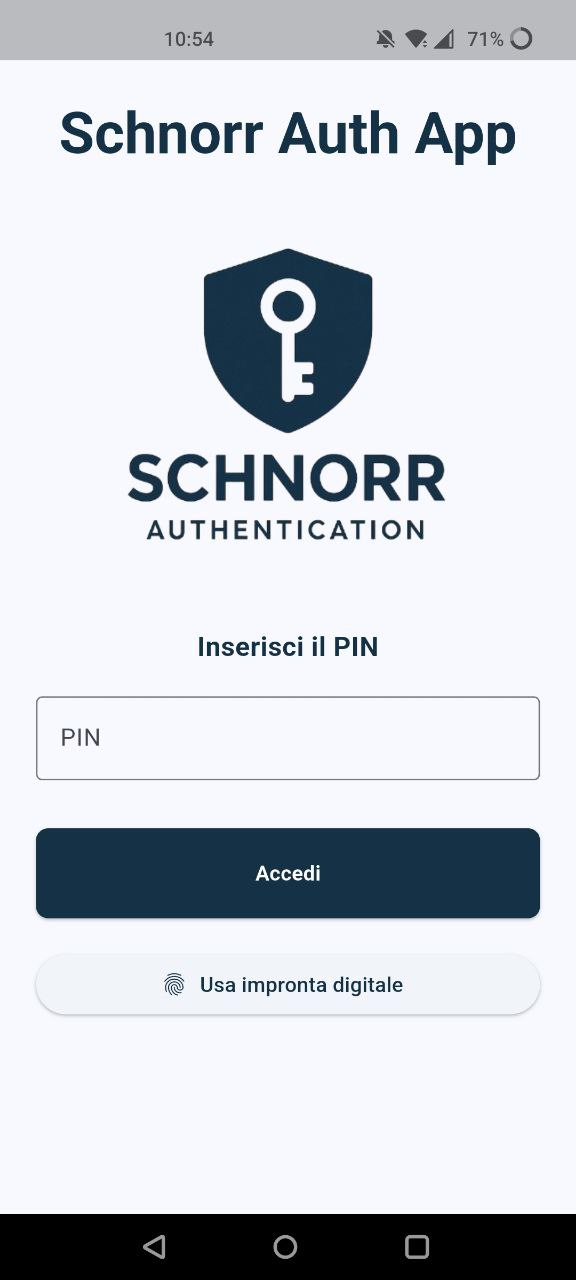
\includegraphics[width=\textwidth]{images/welcome.jpg}
        \caption{Schermata iniziale nella quale impostare il PIN.}
        \label{fig:welcome}
    \end{minipage}\hfill
    \begin{minipage}{0.45\textwidth}
        \centering
        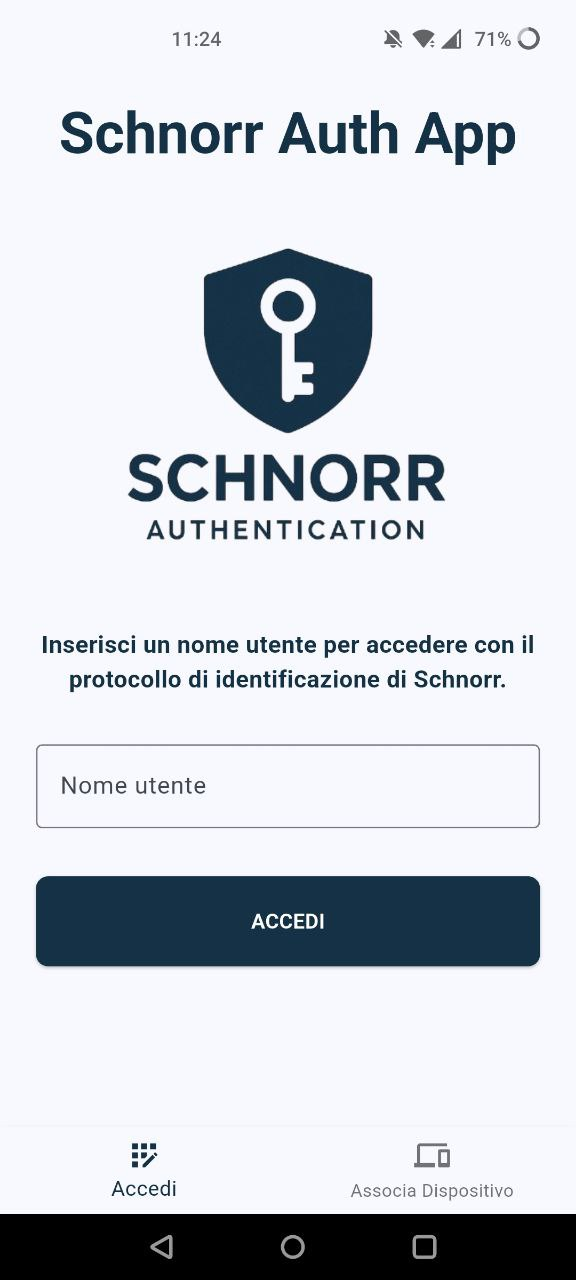
\includegraphics[width=\textwidth]{images/auth.jpg}
        \caption{Fase di registrazione/autenticazione.}
        \label{fig:auth}
    \end{minipage}
\end{figure}

\begin{figure}[h!]
    \centering
    \begin{minipage}{0.45\textwidth}
        \centering
        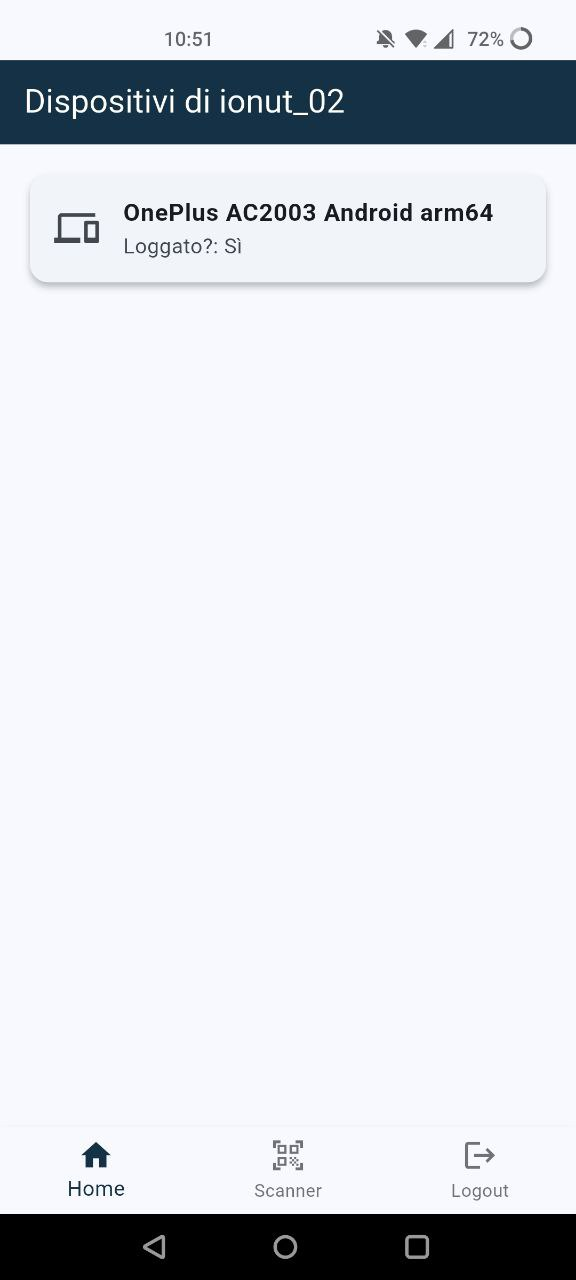
\includegraphics[width=\textwidth]{images/devices.jpg}
        \caption{Pagina principale con dispositivi associati.}
        \label{fig:devices}
    \end{minipage}\hfill
    \begin{minipage}{0.45\textwidth}
        \centering
        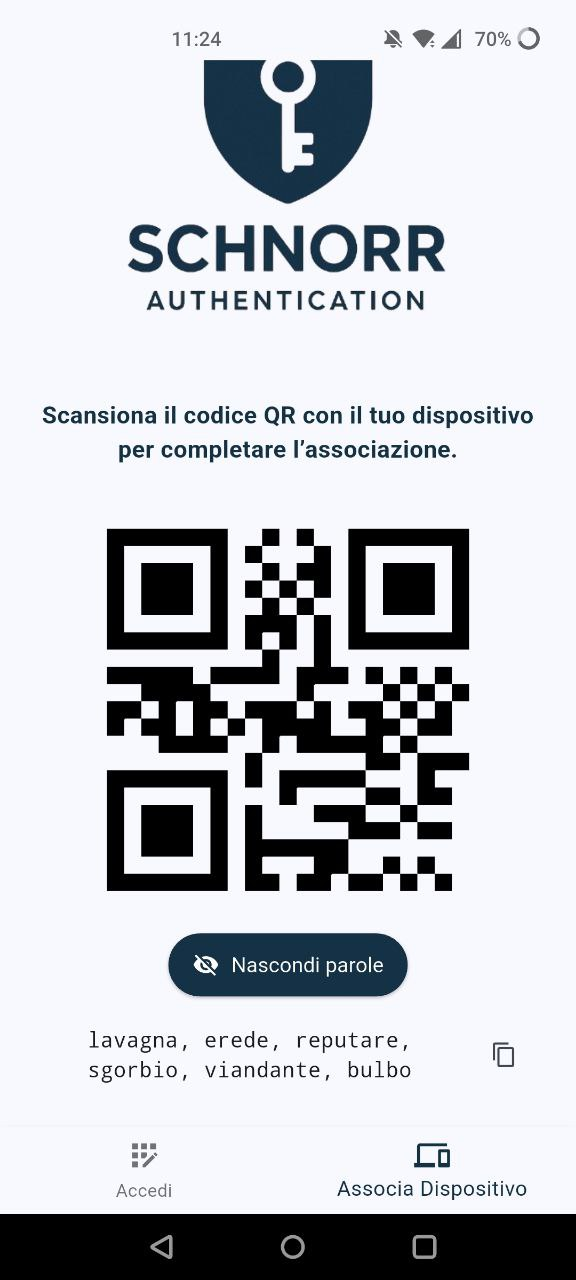
\includegraphics[width=\textwidth]{images/req.jpg}
        \caption{Pagina con QR code e parole.}
        \label{fig:qr_code}
    \end{minipage}
\end{figure}

\chapter{Conclusioni e Sviluppi Futuri}

Il presente capitolo ha la funzione di raccogliere le considerazioni conclusive relative al lavoro di ricerca e sviluppo svolto. L'elaborato si è mosso a partire da una fase di studio teorico sui protocolli di \textit{Zero Knowledge Proof}, passando in seguito alla loro sottoclasse dei protocolli Sigma, per poi concentrarsi in maniera specifica sul protocollo di identificazione di Schnorr. Di quest'ultimo sono stati analizzati sia il meccanismo di autenticazione interattiva, sia l'adattamento che consente di derivarne uno schema di firma digitale. Tale percorso ha fornito le basi concettuali necessarie per la progettazione e realizzazione dell'applicazione \textit{SchnorrAuthApp},
che integra questi principi in un contesto applicativo concreto.

Nonostante l'elevato livello di sicurezza garantito da un protocollo di autenticazione basato su meccanismi di \textit{Zero Knowledge Proof} (ZKP), la sua adozione in contesti reali risulta ancora complessa. I protocolli di autenticazione standard, come PAP o CHAP, continuano infatti a essere ampiamente utilizzati, poiché offrono un compromesso ritenuto accettabile tra sicurezza, semplicità di implementazione e facilità d'uso. Di conseguenza, i protocolli ZKP, pur rappresentando una soluzione tecnologicamente più avanzata, faticano a trovare un impiego diffuso al di fuori di scenari sperimentali o ambiti in cui la sicurezza riveste un'importanza critica.

L'applicazione sviluppata rappresenta comunque un risultato significativo, poiché dimostra la fattibilità tecnica di un sistema di autenticazione fondato su principi crittografici avanzati. \textit{SchnorrAuthApp} traduce in termini concreti e operativi un modello teorico complesso, mostrando come i protocolli ZKP possano essere implementati in modo efficace anche in ambienti mobili e multipiattaforma, grazie al framework Flutter. La pubblicazione del codice sorgente su una piattaforma open source come GitLab contribuisce inoltre alla trasparenza e alla riproducibilità del lavoro, favorendo la collaborazione e la possibilità di ulteriori evoluzioni da parte della comunità.

Durante lo sviluppo sono emerse tuttavia alcune sfide tecniche e concettuali. Una delle principali difficoltà è legata alla gestione sicura delle chiavi crittografiche, in particolare nei contesti mobili dove la persistenza dei dati e la protezione dell'ambiente di esecuzione non sono sempre garantite. Allo stesso modo, l'esigenza di bilanciare sicurezza e usabilità rappresenta un aspetto centrale: un sistema di autenticazione, per essere realmente adottato, deve infatti risultare semplice da usare e da integrare con le infrastrutture esistenti. Inoltre, la mancanza di standard consolidati per l'integrazione dei protocolli ZKP nei framework di autenticazione più diffusi (come OAuth 2.0 o OpenID Connect) costituisce un ulteriore ostacolo alla loro diffusione su larga scala.

\section{Possibili Sviluppi Futuri}

Gli sviluppi futuri del progetto potranno concentrarsi su diverse direzioni. Un primo passo potrà consistere nell'integrazione del protocollo di Schnorr con architetture di autenticazione standard, in modo da ampliare la compatibilità del sistema con applicazioni web e servizi distribuiti.
Un'evoluzione naturale del progetto potrebbe consistere nell'integrazione del sistema di autenticazione basato sul protocollo di Schnorr all'interno di un server web, come componente o plugin di librerie e framework HTTP comunemente utilizzati nello sviluppo di applicazioni web. In questo modo, il protocollo potrebbe essere impiegato non solo per l'autenticazione degli utenti, ma anche per la protezione delle API, offrendo un'alternativa sicura ai tradizionali meccanismi basati su token o password. Una tale integrazione permetterebbe di estendere l'utilizzo del sistema a contesti reali e distribuiti, sfruttando l'interoperabilità offerta dai principali linguaggi di programmazione e framework moderni.

Un'ulteriore estensione potrebbe riguardare l'introduzione di una funzionalità per l'esportazione e l'importazione sicura della chiave privata, utile a creare copie di backup protette.
In questo modo, un utente che dispone di un solo dispositivo avrebbe la possibilità di salvare la propria chiave segreta su un supporto esterno, come un hard drive, senza comprometterne la sicurezza.
Tale meccanismo garantirebbe una maggiore resilienza ai guasti o alla perdita del dispositivo principale, mantenendo al contempo la riservatezza della chiave segreta.


\bibliographystyle{ieeetr}
\bibliography{refs}
\addcontentsline{toc}{chapter}{BIBLIOGRAFIA}
%=========================================================
% APPENDICE
%=========================================================
\appendix
\chapter[APPENDICE]{Codice sorgente}

Questa appendice raccoglie il codice sorgente principale relativo alle componenti
implementative del protocollo di autenticazione basato su Schnorr.  
Le classi riportate rappresentano i moduli centrali per la gestione delle chiavi crittografiche
e per l'esecuzione delle fasi di prova e verifica all'interno del protocollo.

%---------------------------------------------------------
\section{\texttt{KeyManager}}
\label{sec:key_manager}
%---------------------------------------------------------

La classe \texttt{KeyManager} gestisce la memorizzazione sicura delle chiavi private
degli utenti. Se viene fornita una password, la chiave viene cifrata con AES-GCM
utilizzando una chiave derivata tramite Scrypt. In assenza di password, la chiave
viene salvata in chiaro nel file system locale.

\begin{listing}
\begin{minted}[
    frame=lines,
    linenos,
    breaklines,
    fontsize=\fontsize{9pt}{11pt}\selectfont
]{python}
import os
import cryptography
from pathlib import Path
from cryptography.hazmat.primitives.kdf.scrypt import Scrypt
from cryptography.hazmat.primitives.ciphers.aead import AESGCM

class KeyManager:
    HOME_PATH = Path.home()
    SCHNORR_DIR = HOME_PATH / ".schnorr"

    @staticmethod
    def _derive_key(password: str, salt: bytes) -> bytes:
        """Deriva una chiave AES-256 (32 byte) usando PBKDF2-HMAC-SHA256"""
        ...
    
    @classmethod
    def save_private_key(cls, username: str, key: int, password: str = None) -> None:
        cls.SCHNORR_DIR.mkdir(parents=True, exist_ok=True)
        privkey_path = cls.SCHNORR_DIR / f"{username}_privkey.pem"

        if not password:
            cls._save_private_key(username, key)
            return

        data = str(key).encode()
        salt, nonce = os.urandom(16), os.urandom(12)
        aesgcm = AESGCM(cls._derive_key(password, salt))
        ciphertext = aesgcm.encrypt(nonce, data, None)
        with open(privkey_path, "wb") as f:
            f.write(salt + nonce + ciphertext)

    @classmethod
    def load_private_key(cls, username: str, password: str = None) -> int:
        privkey_path = cls.SCHNORR_DIR / f"{username}_privkey.pem"

        if not password:
            return cls._load_private_key(username)

        with open(privkey_path, "rb") as f:
            blob = f.read()
        salt, nonce, ciphertext = blob[:16], blob[16:28], blob[28:]
        aesgcm = AESGCM(cls._derive_key(password, salt))
        plaintext = aesgcm.decrypt(nonce, ciphertext, None)
        return int(plaintext.decode())
\end{minted}
\caption{Implementazione della classe \texttt{KeyManager}.}
\end{listing}

%---------------------------------------------------------
\section{\texttt{SchnorrProver} e \texttt{SchnorrVerifier}}
\label{sec:schnorr_classi}
%---------------------------------------------------------

Le classi \texttt{SchnorrProver} e \texttt{SchnorrVerifier} implementano rispettivamente
il ruolo del Prover e del Verifier nel protocollo di identificazione di Schnorr.
La prima gestisce la generazione delle chiavi e la produzione della risposta,
mentre la seconda verifica la validità della prova o della firma associata.

\begin{listing}
\begin{minted}[
    frame=lines,
    linenos,
    breaklines,
    fontsize=\fontsize{8.5pt}{10pt}\selectfont
]{python}
class Schnorr:
    def __init__(self, group_id: GroupType):
        self.crypto_group = Rfc3526(group_id)
        self.p, self.g, self.q = self.crypto_group.get_params()
        self.public_key, self.public_key_temp = None, None

    def compute_challenge(self, message: int) -> int:
        data = str(self.public_key_temp) + str(self.public_key) + message
        return int(hashlib.sha256(data.encode()).hexdigest(), 16) % self.q

class SchnorrProver(Schnorr):
    def __init__(self, group_id: GroupType):
        super().__init__(group_id, filename)
        self.alpha, self.alpha_temp = None, None
        
    def public_key(self) -> int:
        if self.public_key is None:
            self.public_key = pow(self.g, self.alpha, self.p)
        return self.public_key

    def public_key_temp(self) -> int:
        self.alpha_temp = random.randint(1, self.q - 1)
        self.public_key_temp = pow(self.g, self.alpha_temp, self.p)
        return self.public_key_temp

    def gen_keys(self):
        self.alpha = random.randint(1, self.q - 1)
        self.public_key = pow(self.g, self.alpha, self.p)

    def response(self, challenge: int) -> int:
        return (self.alpha_temp + self.alpha * challenge) % self.q

    def sign_message(self, message: str) -> dict[str, int]:
        challenge = self.compute_challenge(message)
        sign = {"public_key_temp": self.public_key_temp, "response": self.response(challenge)}
        return sign
        
class SchnorrVerifier(Schnorr):
    def __init__(self, group_id: GroupType):
        super().__init__(group_id, filename)
        self.challenge = random.randint(0, self._q - 1)

    def check(self, response: int) -> bool:
        left = pow(self.g, response, self.p)
        right = (self.public_key_temp * pow(self.public_key, self.challenge, self.p)) % self.p
        return left == right
    
    def verify_sign(self, sign: dict, message: str) -> bool:
        self.public_key_temp = sign["public_key_temp"]
        self.challenge = self.compute_challenge(message)
        return self.check(sign["response"])
\end{minted}
\caption{Classi \texttt{SchnorrProver} e \texttt{SchnorrVerifier}.}
\end{listing}

\clearpage


\end{document}
